\graphicspath{{chapters/05_results/images}}
\chapter{Results}

% The Results part describes all the experiments performed and their statistical analysis (at least 10, maximum 40 pages). If you want to provide replication data, include them in another appendix (Appendix II).

This chapter will focus on benchmarking the preprocessing procedure implemented by HiCONA, computing various statistics at different steps, measuring time and memory performance, as well as performing some biological validation via replicate correlation. For some steps, HiCONA will also be compared to loop-callers, meaning tools which try to identify pixels corresponding to loop domains using various approaches. Though loop-callers do not have the exact same objective as HiCONA, they will still be used as reference since they are the only tools found in literature which could reasonably fulfill this role. No network analysis proper will be presented, since the algorithms are still being implemented and tested, though some preliminary results will be mentioned in the discussion.

Unless specified otherwise, all the data and analyses shown in this chapter were performed by my tutor, Leonardo Morelli, using HiCONA, which I implemented, as well as other custom scripts. The comparison with cooltools and the benchmarking were performed by me; moreover, I adapted all the analyses and plots to highlight aspects relevant to the way HiCONA was implemented.

\section{Pixel preprocessing steps analysis}

The objective of preprocessing is to create chromosome-level networks and reduce their density using network sparsification, that is, extracting the backbone composed of the most significant interactions while also preserving topology. Moreover, since the network has a biological meaning, there are other characteristics that could be kept into account; one such characteristic is the distribution of the genomic distances of the edges, i.e. the pixels. For instance, one could try and preserve this distribution, meaning that the preprocessing procedure should remove, for each genomic distance, an amount of pixels proportional to the initial fraction of pixels with that distance; this would guarantee that the algorithm is not biased in favor of some genomic distance. This objective cannot be achieved with a method such as network sparsification, since genomic distance is not taken into account during the sparsification step; still, it is worth keeping track of mean and median genomic distance at each step to guide in the choice of parameters to use and in general to analyze algorithm behavior. 

With this in mind, the individual processing steps will be analyzed. Firstly, distance normalization will be discussed, then pixel filtering. This is because, though some filtering steps do happen prior to normalization, the last filter is applied on normalized counts; thus, it seems more clear to tackle filtering all at once. Then, network sparsification will be discussed. 

As another remark, each preprocessing function works with exactly one chromosome at a time. The chromosomes are fully independent from each other throughout the entirety of the preprocessing (and, in the future, of the analysis); this can make it quite difficult to aggregate the data coming from all the chromosomes of an individual processed file. For this reason, data will be aggregated when possible; when no convenient way is found, one chromosome from one of the files will be used as an example, and the same analysis conducted on at least another random chromosome of the same file, as well as on a random chromosome from another file, will also be included in the Appendix II as replication data.

\subsection{Normalization factor computation}

Pixels whose bins are close in the genome tend to have significantly higher counts than pixels whose bins are far apart, simply due to random interactions; it is thus needed to penalize short-range interactions to allow for a fair pixel comparison during filtering and sparsification. In order to normalize for genomic distance, it is necessary to compute some summary statistic $P(d)$, with $d$ being genomic distance, to use as normalization factor (i.e. denominator of a fold change); here we compare the statistics obtained using \textit{cooltools} and HiCONA (for the formulas refer to subsection \ref{par:distnorm}). 

% Plot of Hicona expected count vs cooltool ones
\begin{figure}[ht]
  \centering
  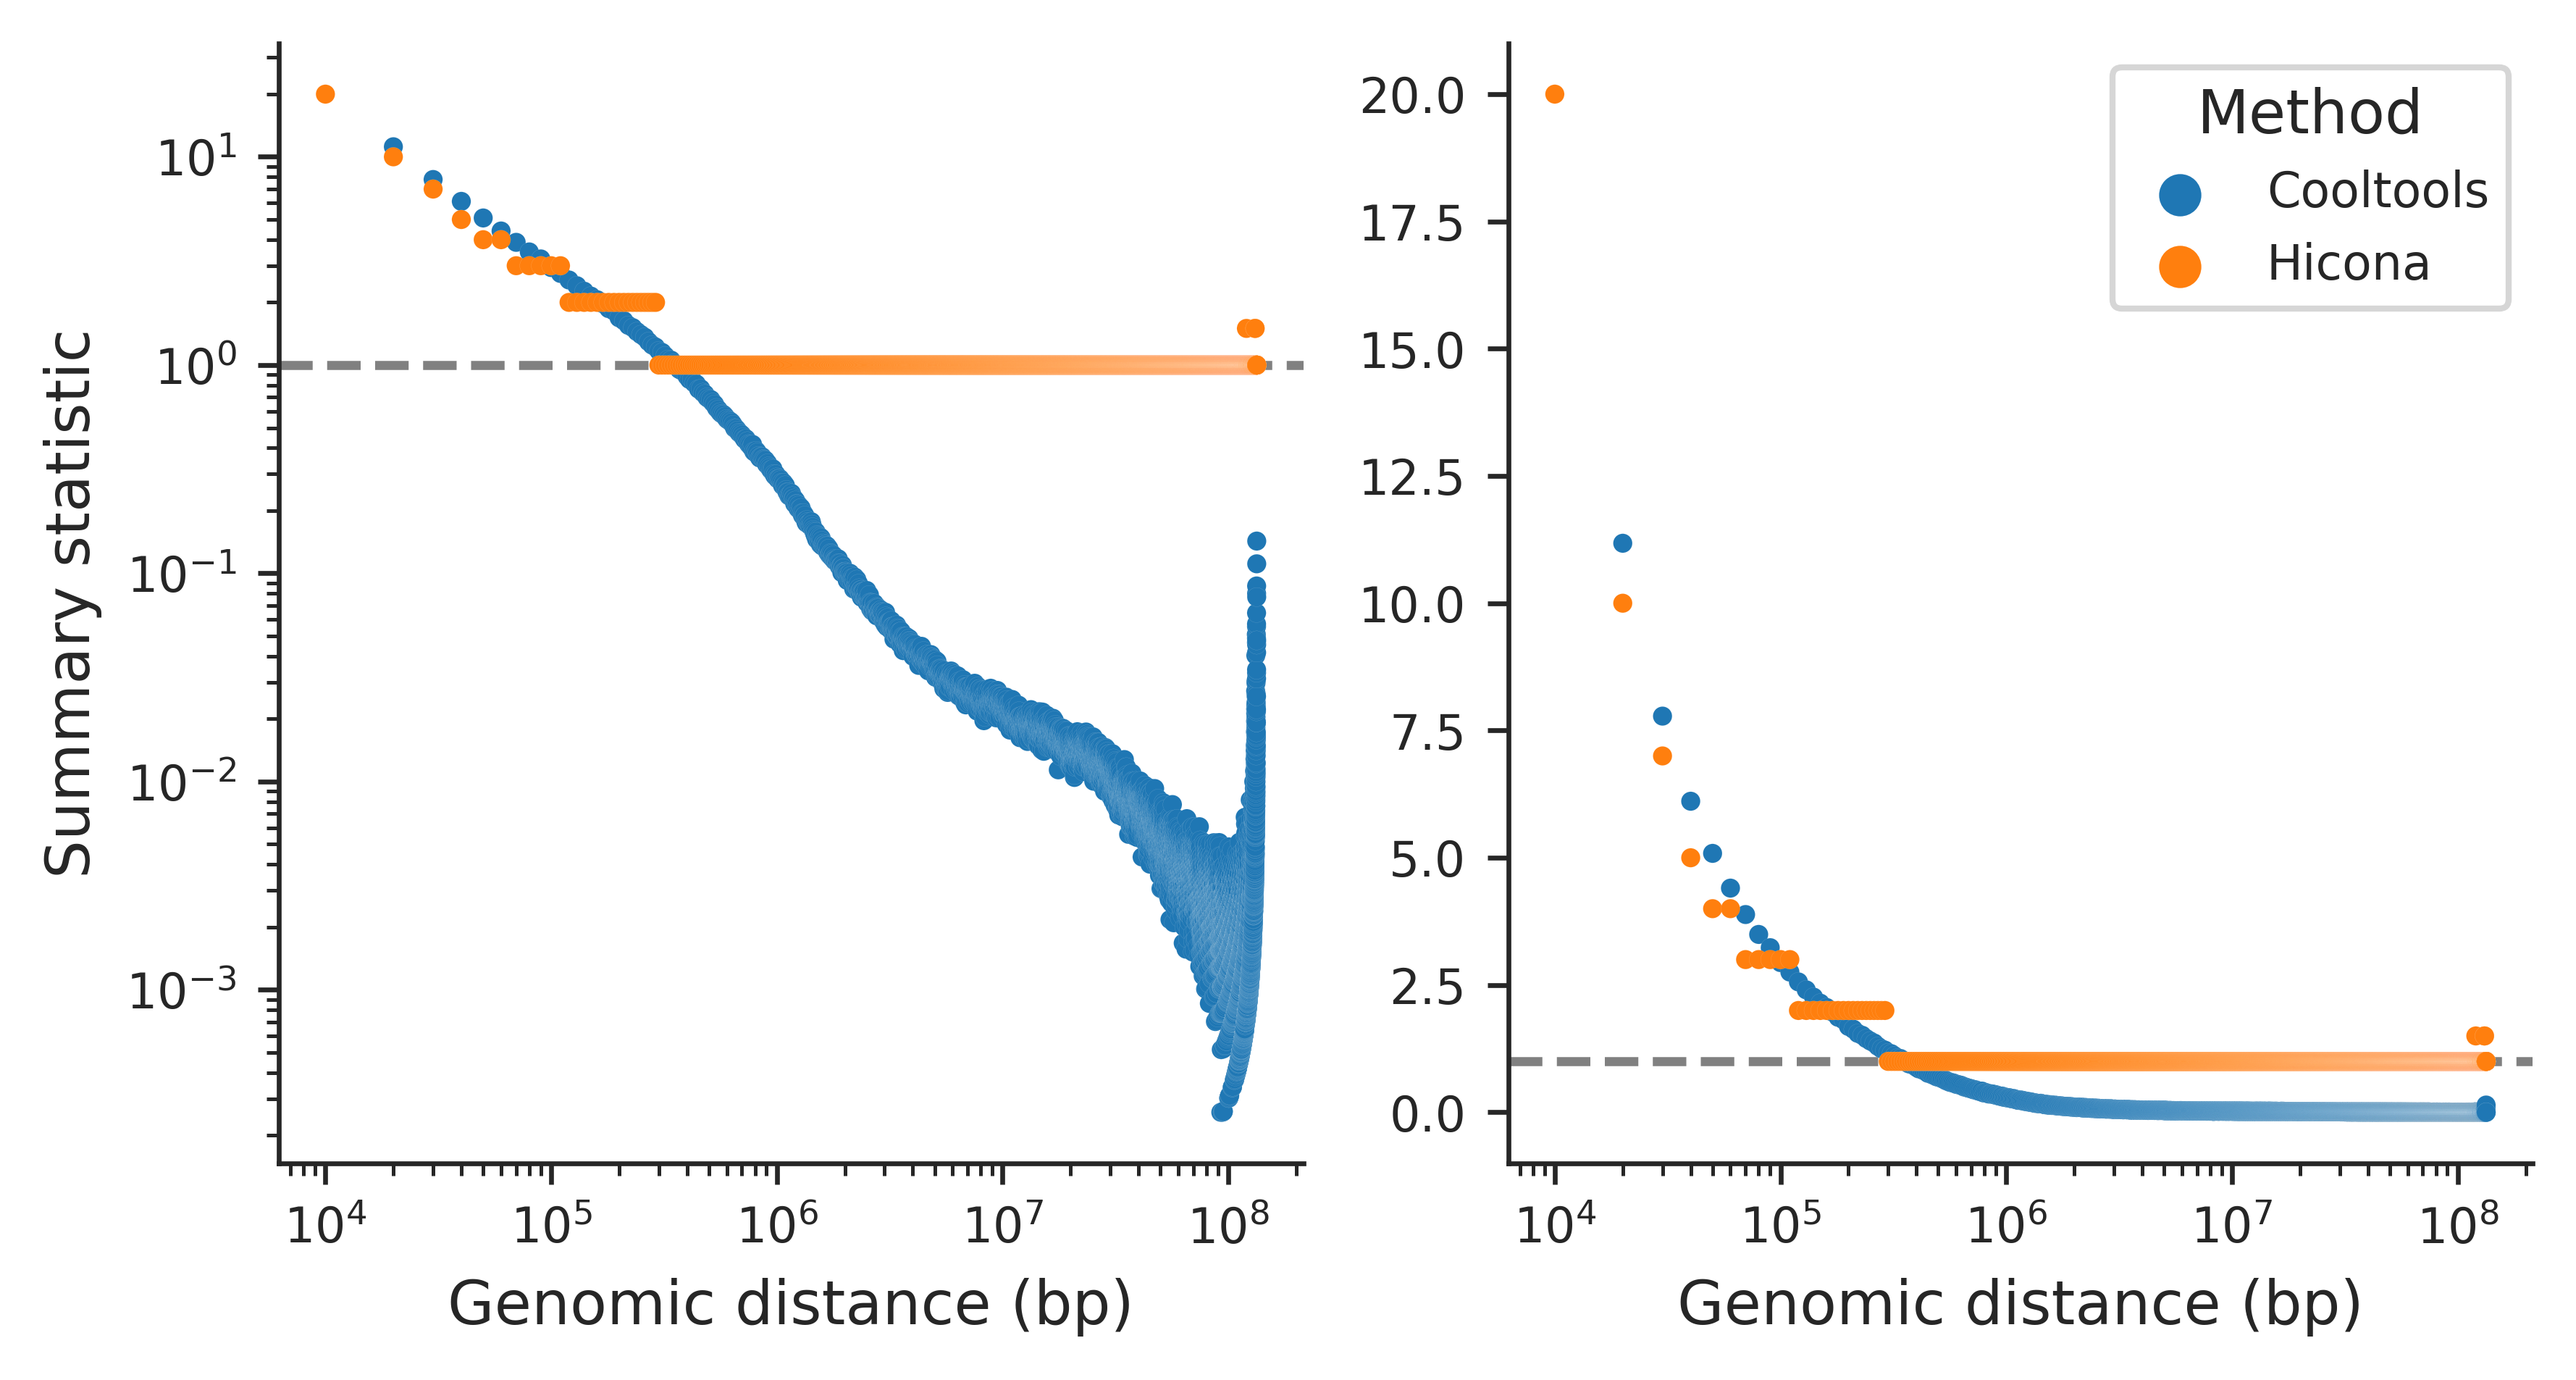
\includegraphics[width=1\textwidth]{hicona_vs_cooltools.png}
  \caption{\textbf{Comparison of summary statistics from HiCONA and cooltools}. Comparison of the genomic distance normalization factors for chromosome 1 of IMR90 cells, at 10 kb resolution, filtered using 200 Mb as genomic distance threshold, obtained using HiCONA and cooltools. On the left, normalization factor with respect to distance in log-log scale, on the right the same plot but without log-transform of the y-axis.}
  \label{fig:cooltools}
\end{figure}

As previously mentioned, the probability of two genomic regions interacting by chance decays exponentially with their distance from each other; for this reason, we also expect the function describing probability of contact given distance to be linear in a log-log plot. As shown in the left panel of figure \ref{fig:cooltools}, the summary statistic provided by \textit{cooltools} can indeed be considered linear for a big range of genomic distances (up to $10^7$ bp); for very high distances though, we start observing some fanning which represents instability due to the low number of pixels averaged. This happens not only because the number of interactions decays with distance, but also because the number of theoretically possible pixels decreases. Visually, increasing distance means moving from the main diagonal of the contact matrix to diagonals closer to the upper right corner, which become shorter and shorter. \textit{Cooltools} allows to address this instability with a smoothing procedure, though it currently requires matrix balancing, which introduces the assumption that all genomic loci form the same number of contacts. In synthesis, the procedure adopted by \textit{cooltools} is biologically sensible, though it has some drawbacks such as very low counts and instability at very high distances.


The summary statistic proposed by HiCONA, instead, is not linear in the log-log plot. At low distances it behaves similarly to \textit{cooltools}, but then it plateaus at 1 (or if a minimum count threshold is imposed, the cutoff itself becomes the plateau value). Though at first glance the two methods seem rather different, this is mostly due to the logarithmic scale of the y-axis. The right panel of figure \ref{fig:cooltools} represents the same plot but with the y-axis in linear scale; from this we notice that the values provided by the two methods are actually quite close, since \textit{cooltools} tends asymptotically to 0, while HiCONA is stable at 1 (with some rare exceptions at extremely high distances). Moreover, it must be considered that non-normalized pixel counts are integers strictly greater than zero, therefore the minimum value which they can take is 1; by using a number close to zero as summary statistic, and thus to compute a fold change, a pixel with count 1 at high distance will seem extremely significant, though it might be due to a single random ligation event. The statistic provided by HiCONA is therefore similar to the biologically motivated one provided by \textit{cooltools}, though with the advantage of being more stable and yielding integer values.


\subsection{Genomic distance normalization}

After computing the normalization factors, the pixels are normalized (see subsection \ref{par:distnorm} for the exact formula). This means that pixels whose count is equal to the expected one will have normalized value equal to 1; any value above 1 means higher count than the expected, any value below 1 means lower count than the expected. 

% Plot from first lab meeting with distribution prior and after normalization
\begin{figure}[ht]
  \centering
  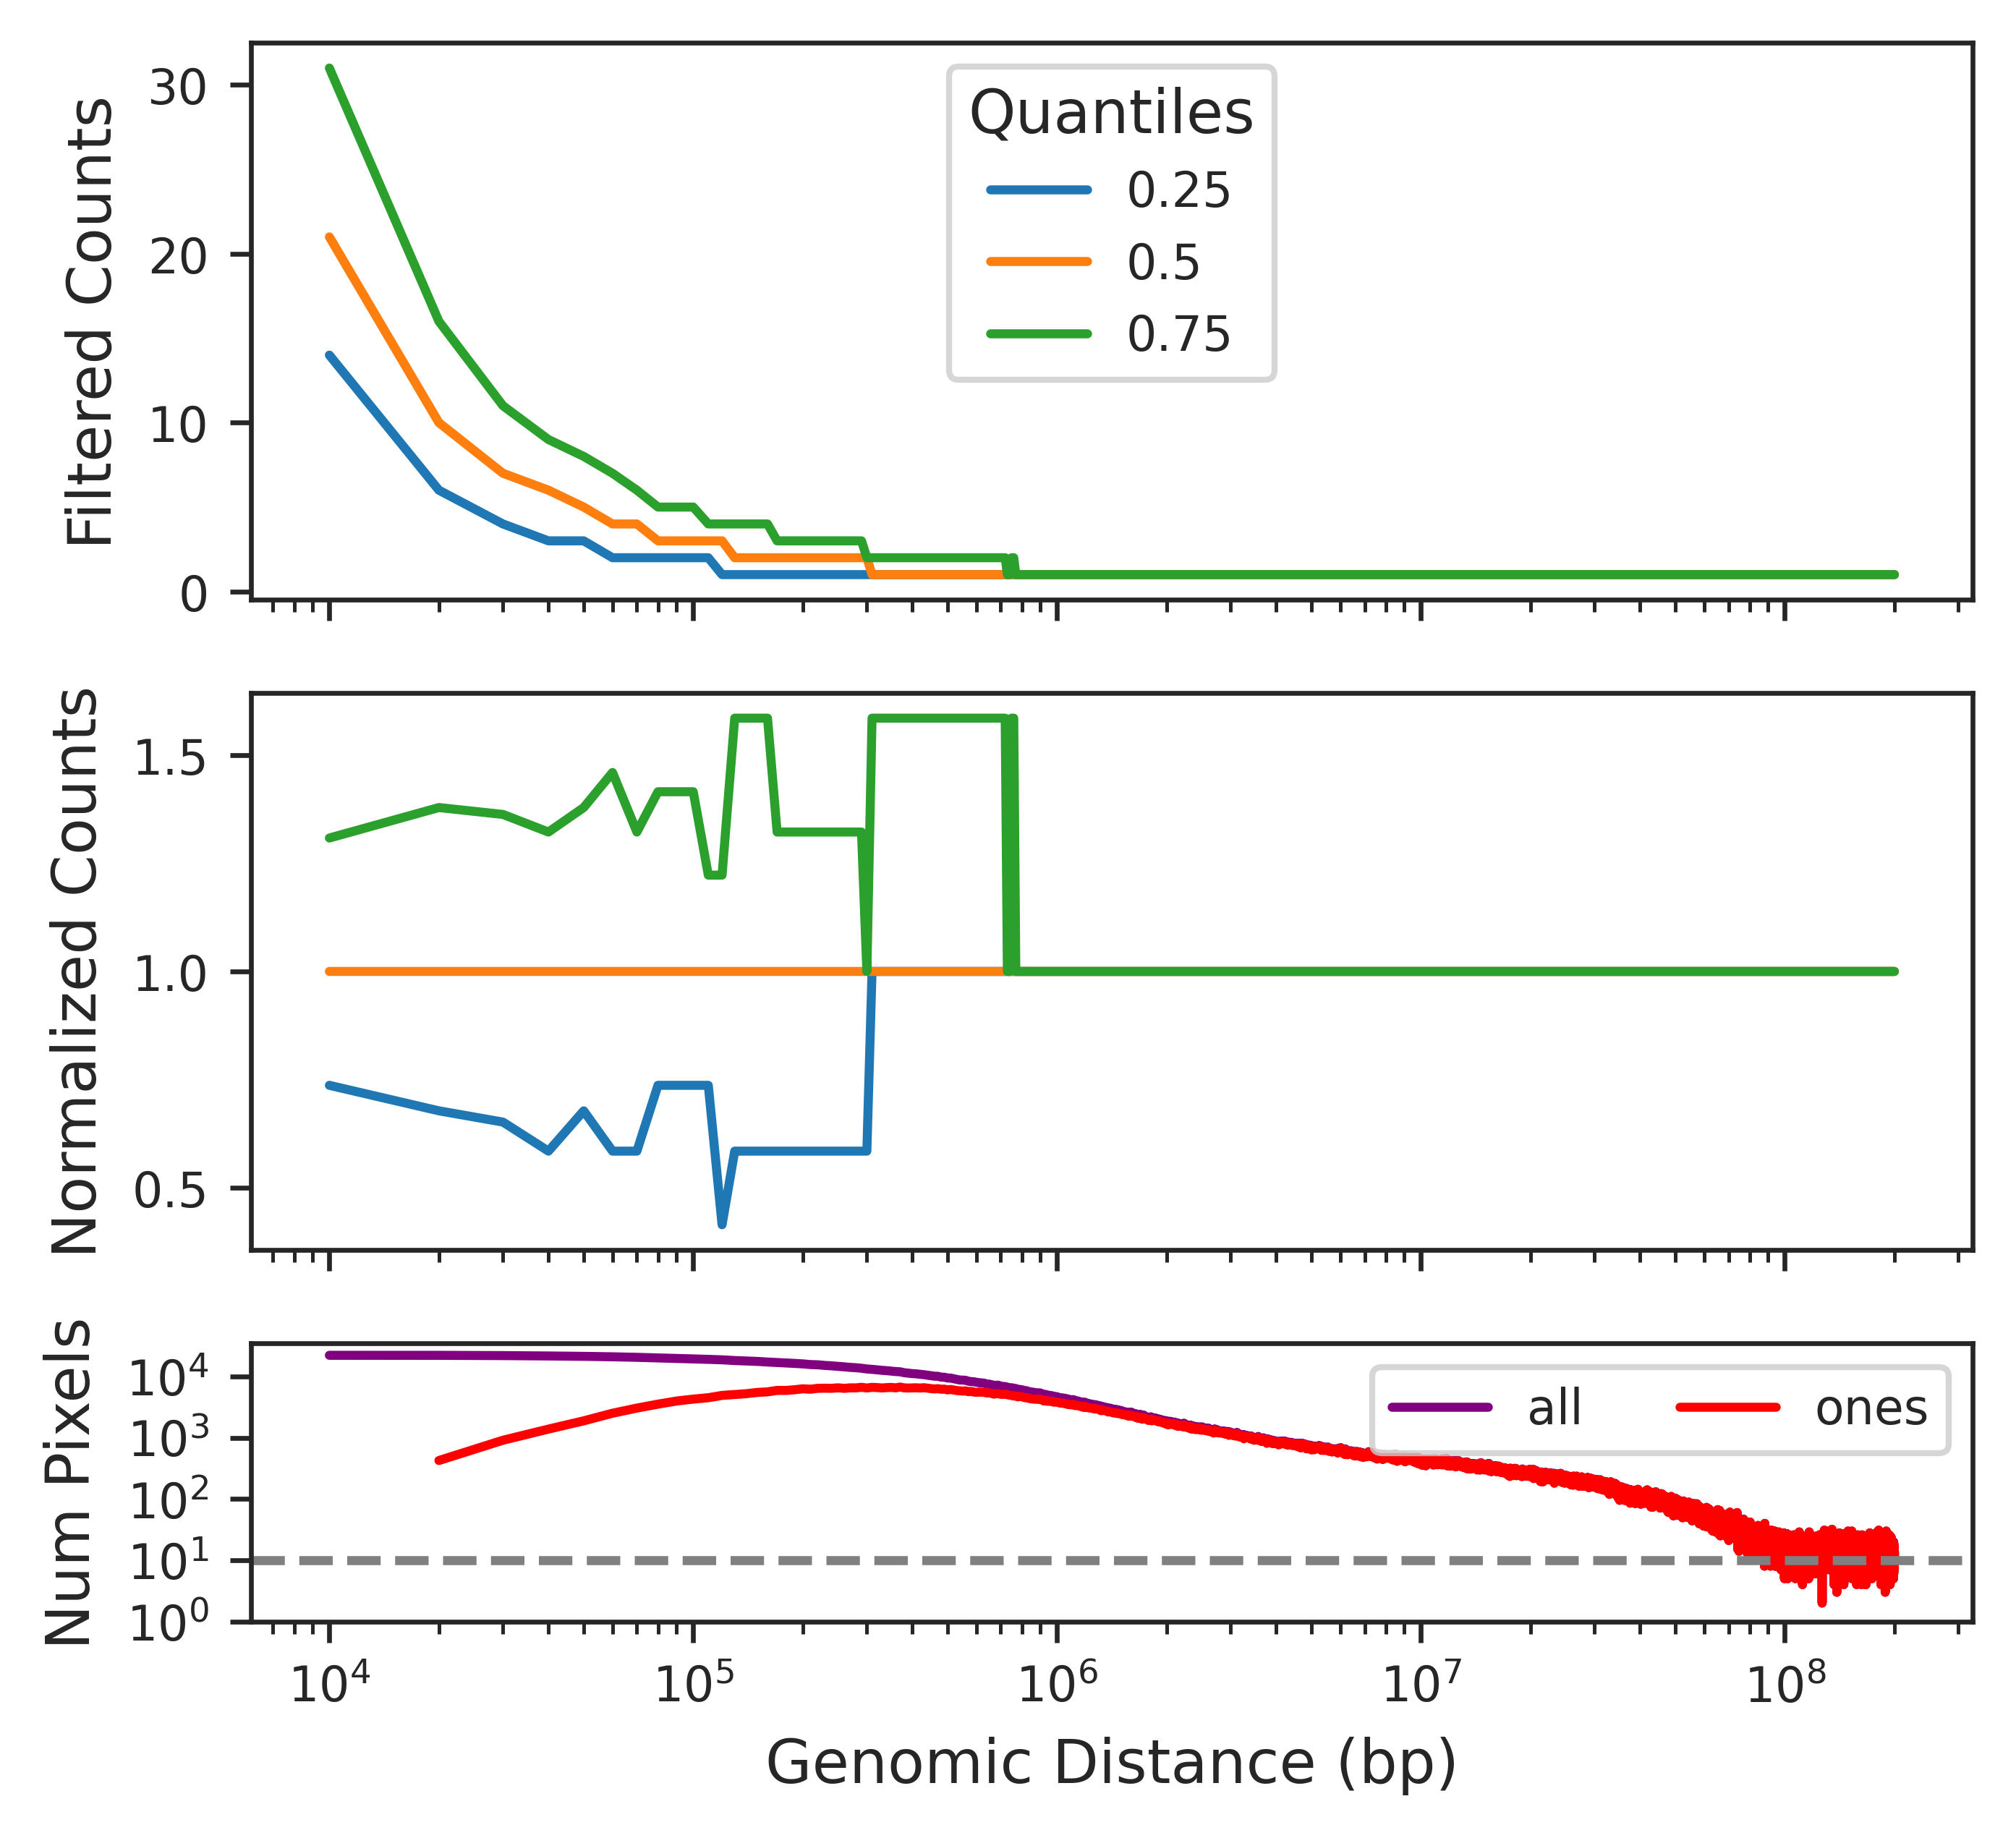
\includegraphics[width=0.7\textwidth]{normalization_stats.png}
  \caption{\textbf{Comparison of pixels counts distribution prior and post genomic distance normalization}. Comparison of the distribution of raw and normalized counts at each genomic distance for chromosome 1 of IMR90 cells, at 10 kb resolution, filtered using 200 Mb as genomic distance threshold. At the top, quantiles of the raw counts distribution for each genomic distance. In the middle, quantiles of the normalized counts distribution for each genomic distance. At the bottom, total number of pixels, and number of pixels with raw count equal to 1, for each genomic distance.}
  \label{fig:normstats}
\end{figure}

In figure \ref{fig:normstats} we can observe how the counts distribution changes with normalization. In the top panel, the quantiles of the raw counts distribution for each genomic distance are shown. Though the median of the raw counts distribution can start at different values, in this case 22, it always quickly converges to 1, regardless of chromosome and file. This behavior can also be justified by looking at the bottom panel, which shows the total number of pixels, and the number of pixels with raw count equal to 1, as a function of genomic distance. While the number of pixels quickly decreases with distance, to the point where there are less than 100 at $10^8$ bp, the fraction of them with raw count equal to 1 rapidly increases; at $10^6$ bp, basically all pixels have raw count equal to 1, thus motivating the median being equal to 1. In the middle panel, the quantiles of the normalized counts distribution for each genomic distance are shown. As one might expect from a normalization process, the value of the median is always 1. Even though the high fraction of raw counts equal to 1 makes it less obvious, on closer inspection it can be seen that the regularization of the spread actually works quite well. Up to $2 \cdot 10^5$ bp, there is a spread in the normalized counts distributions of up to $0.6$ units in either direction of the median. Then, from $2 \cdot 10^5$ to $8 \cdot 10^5$ bp, the same spread of $0.6$ points is present, though only in the positive direction. This it is due to the fact that, at these distances, more than half of the raw counts are equal to 1, as highlighted by the bottom panel and the median in the top one being 1; since 1 is the minimal value that raw counts can take, it means that there are no pixels who can have a raw count below the expected one, and thus a normalized value lower than 1. After $8 \cdot 10^5$ bp, almost all the pixels have raw count equal to 1, thus all quantiles are equal to 1; for this reason it is still impossible to have values lower than 1, and while normalized values above 1 are possible, they are so rare that they do not alter the position of the quantiles except for very high distances. This is to say that, when there is a sufficient amount on pixels with raw count different from 1 to allow for non overlapping quantiles, the amplitude of the spread falls within a very consistent range of one point in either direction, with few distances exceeding this range (regardless of chromosome, cell type, filtering parameters or file size).

\subsection{Pixel filtering}

The preliminary step of pixel filtering is to remove inter-chromosomal pixels. As explained in subsection \ref{par:pixfiltering}, this is because it is not possible to define genomic distance across chromosomes, and therefore these pixels cannot be processed in a comparable way with respect to the intra-chromosomal ones. This step removed, on average, 53.27\% of pixels from the files at 10 kb resolution, 45.62\% of pixels from those at 5 kb resolution.

All the intra-chromosomal pixels for a single chromosome are then filtered. First, self-looping pixels are removed. Subsequently, pixels with genomic distance above a specified threshold are removed. The partially filtered chromosome-level table is then normalized as discussed in the previous subsection. Finally, the normalized table is filtered using a quantile threshold: the value corresponding to a specified quantile of the normalized counts is computed, then all pixels whose normalized counts value is equal to or below it are removed.

In figure \ref{fig:filtering}, some chromosome filtering statistics, aggregated by file, are shown. In each of the panels, the boxes are divided into groups, each one corresponding to a genomic distance threshold, which were sorted from left to right by increasing strictness. Within each group of boxes, each box corresponds to a quantile threshold, once again sorted from left to right in each group by increasing strictness.

In the top panel, the fraction of retained intra-chromosomal pixels after filtering is reported. As expected, both decreasing the distance threshold and increasing the quantile threshold, therefore making the filtering conditions more strict, lead to a decrease in the fraction of retained pixels. While changing distance threshold yields gradual changes in the fraction of retained pixels, changing quantile threshold can cause a quite abrupt drop. This is due to the fact that many pixels, if not most of them, have normalized counts equal to 1. To exemplify this, consider the hypothetical case in which two very distant quantiles, say 0.25 and 0.75, both correspond to a normalized value of 1 due to the sheer number of pixels with that normalized counts value; trying to filter using quantile threshold 0.25 would mean removing all pixels with normalized counts equal to 1, which in turn results in removing all pixels up to the quantile threshold 0.75 since those have normalized counts equal to 1 too, thus causing a drop similar to the one observed in the plot.

In the middle panel, the fold change between the mean genomic distance of the filtered pixels and the mean genomic distance of the non filtered ones is shown. In the bottom panel, the same fold change is represented but using the median instead of the mean. As one might expect, a reduction in both mean and median is observed, which gets progressively bigger as the distance threshold gets smaller. Quantile threshold does not seem to have a big impact on mean and median distance reduction, aside from the drop between 0.05 and 0.1 which is due to the previously mentioned drastic reduction in pixel number. The spread of the mean fold change for a single combination of parameter is quite small, while the spread of the median fold change is quite big; although the spread in median fold change might be due to actual differences in the distribution of genomic distances in the different samples, it is more likely that it is simply due to the way the measure is computed, since it is the ratio among two individual data points (while in the case of the mean, both numerator and denominator are the average of millions of data points).

\begin{figure}[ht]
  \centering
  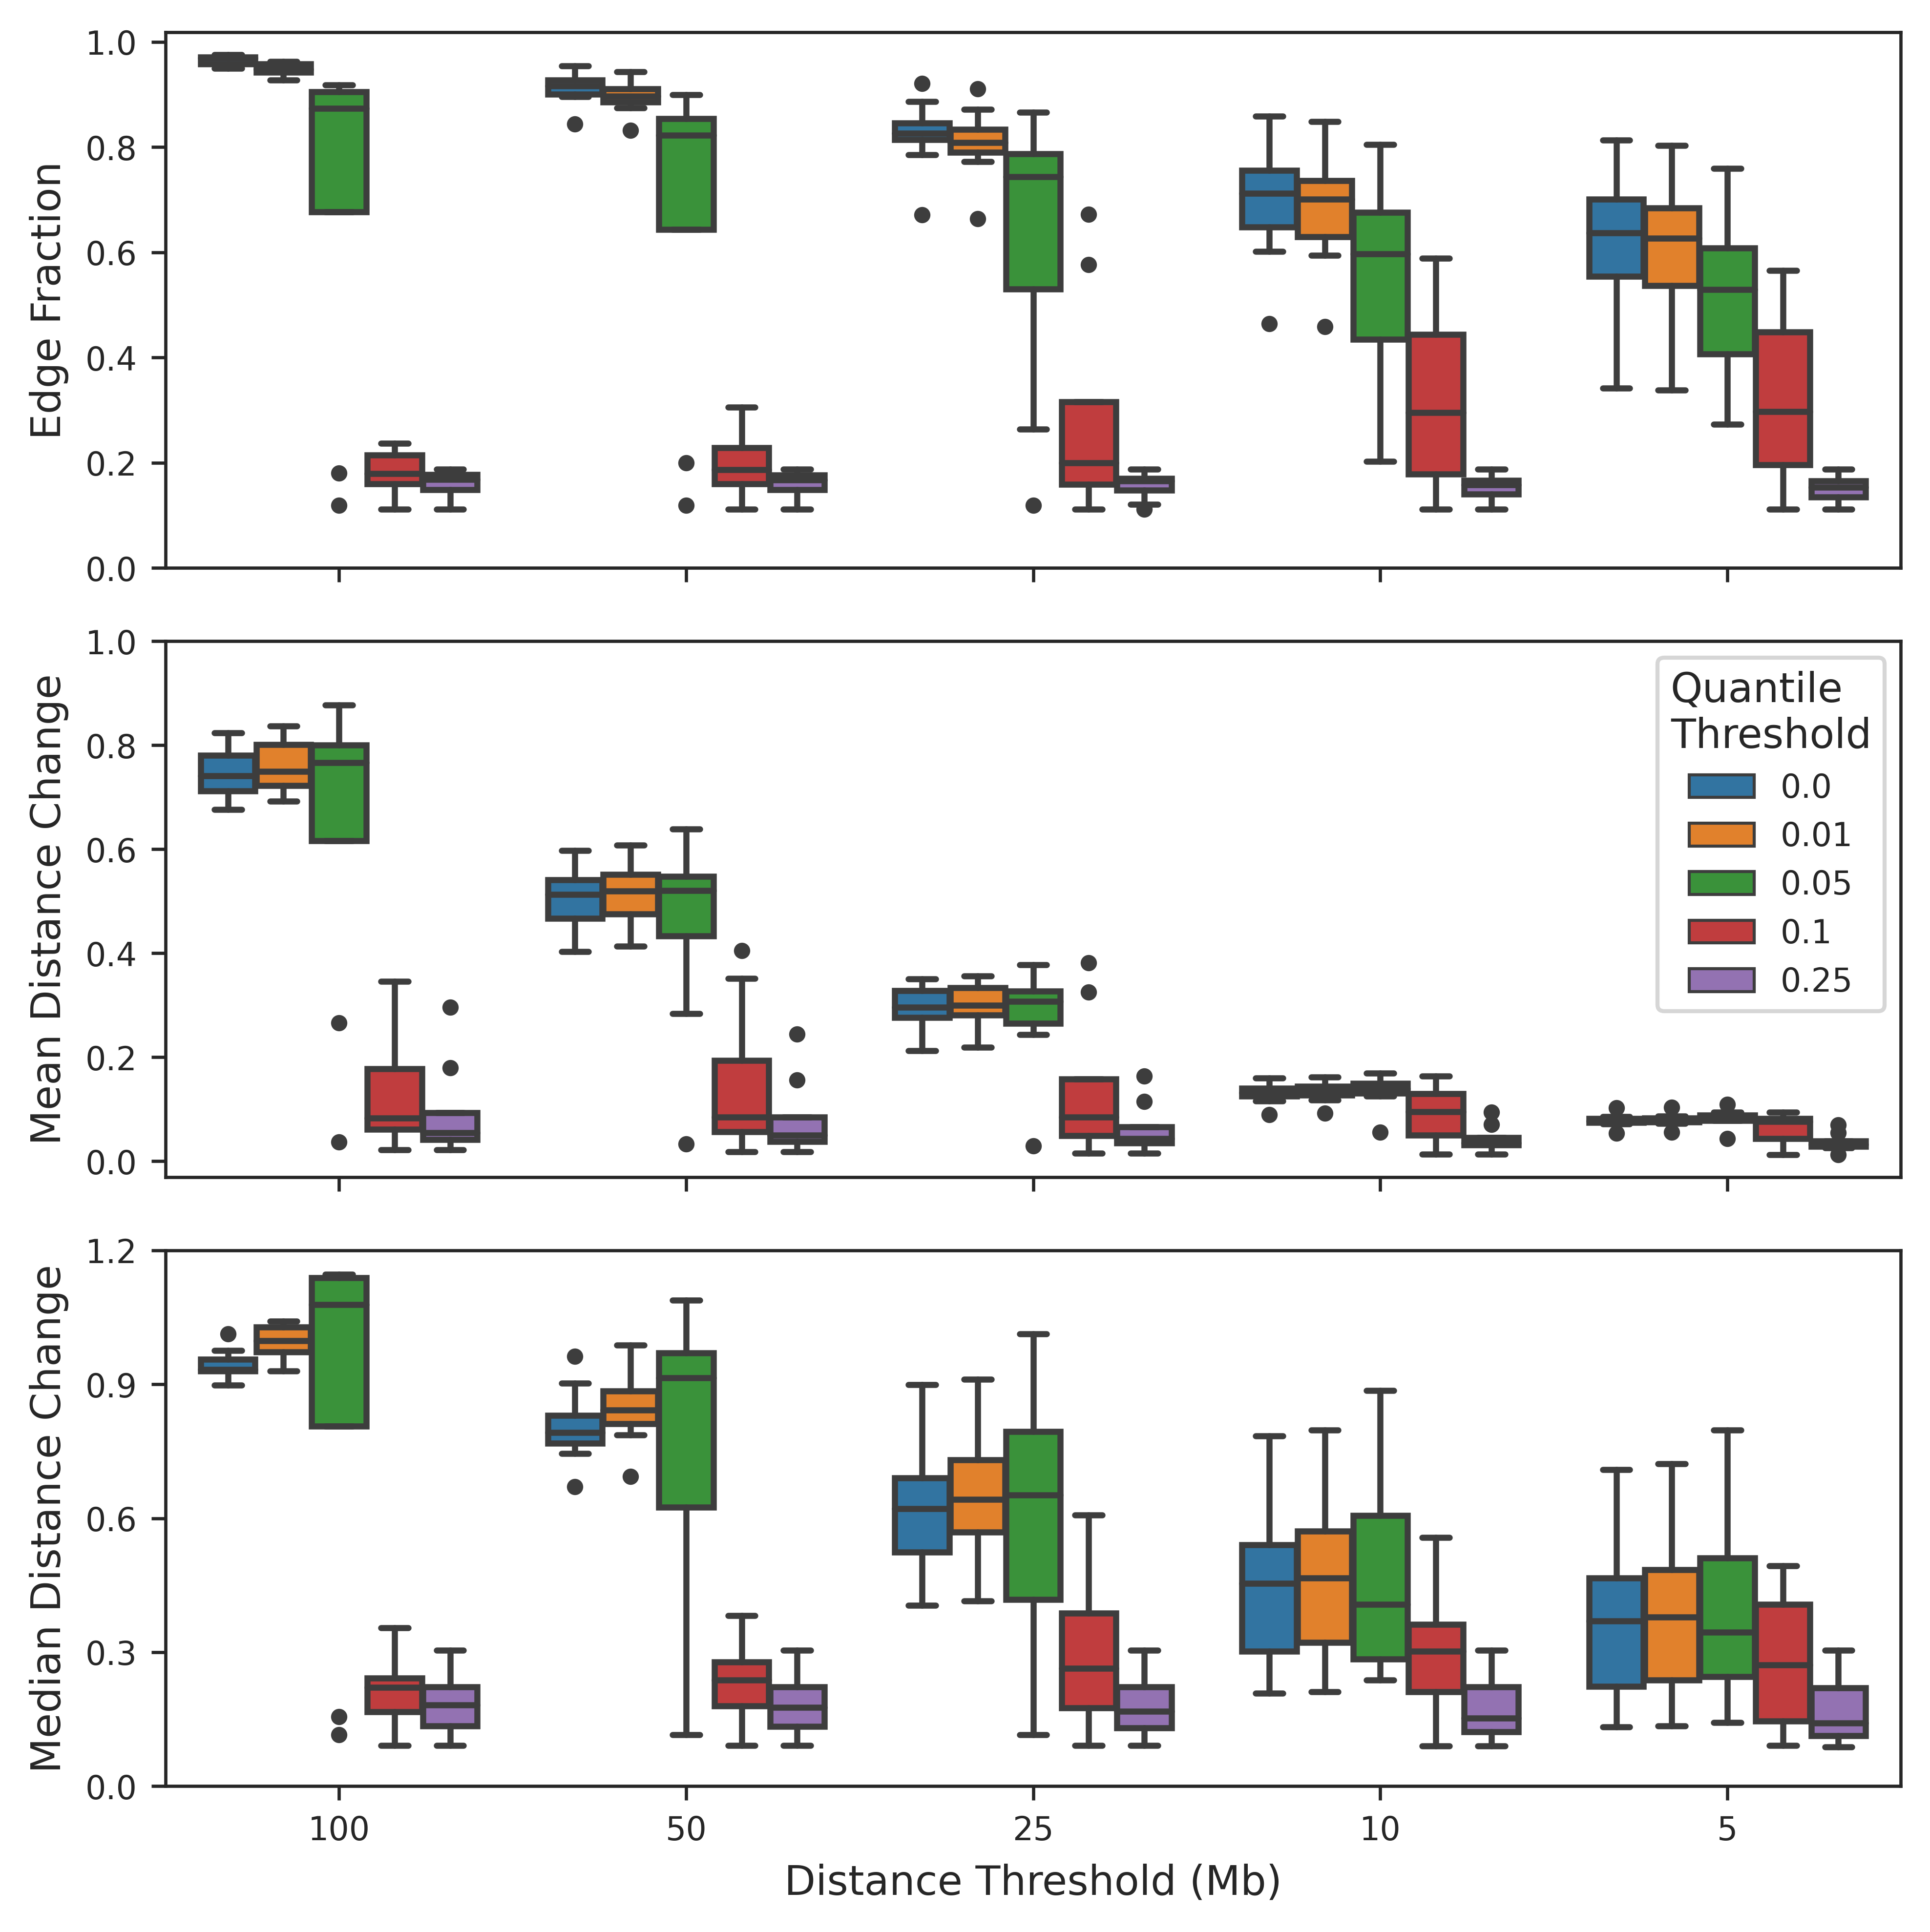
\includegraphics[width=1\textwidth]{filtering_stats.png}
  \caption{\textbf{Changes in pixel number and distance statistics after filtering}. Comparison of the changes in edge number and distance statistics using different filtering parameters on all cool files at 5 kb resolution. Each group of boxes corresponds to one distance threshold, which are sorted from left to right, from least stringent to most stringent. Each box in a group corresponds to one quantile threshold, and within a group, boxes are sorted from left to right, from least stringent to most stringent. At the top, the fraction of intra-chromosomal pixels remaining after filtering. In the middle, fold change between filtered pixels mean genomic distance and intra-chromosomal pixels mean genomic distance. At the bottom, fold change between filtered pixels median genomic distance and intra-chromosomal pixels median genomic distance. The dashed gray line represents the 1 on the y-axis for ease of visualization.}
  \label{fig:filtering}
\end{figure}

Since at this step the edges are still being removed ignoring network properties, it makes sense to apply a filter only if the distance metrics are not heavily altered, and if the filter is consistent in its effect. Given these premises, the only parameter values which seem appropriate are 0.0 and 0.01 for quantile threshold and 100 Mb and 50 Mb for the distance threshold. It is worth noting that 0.0 and 0.01 quantile threshold behave almost identically and that 0.0 corresponds to not applying the filter at all; moreover both 100 Mb and 50 Mb are still very permissive thresholds in terms of genomic distance. This indicates that a filtering step which uses these parameters is not doing much, and it could be removed (aside from the removal of self looping pixels and inter-chromsomal ones).

\newpage
\subsection{Optimal alpha computation}

After pixel filtering, the sparsification scores (or alpha values) are computed for each pixel as discussed in subsection \ref{par:sparscore}. HiCONA computes and stores both alpha values for each edge, in order to be able to use either the minimum or the maximum of the two. To perform the actual sparsification, a sparsification threshold (or alpha cutoff) must be defined. Although an arbitrary one can be chosen, HiCONA gives the option of computing the so-called optimal alpha value, that is the chromosome-level threshold which minimizes the number of edges while maximizing the number of nodes. This value is computed using a local search algorithm; one example of the grid of values tested by a run of the local search is shown in figure \ref{fig:alphas}.

For each chromosome the local search is actually run twice, once using the minimal alphas, once using the maximal ones. For each modality of alpha, a curve is generated from which the corresponding optimal value can be obtained. Typically, the two alpha thresholds for a chromosome are different, though they still tend to be very close to each other ($\pm 0.03$). The typical range for the optimal alpha threshold is between 0.15 and 0.30. Chromosome Y is an exception; either due to the smaller size with respect to the other chromosomes, or possibly due to some difference in biological properties, the curve is too irregular for a reliable estimate. 

% Plot alpha computation grid for some file (maybe multiple sets of params)
\begin{figure}[h]
  \centering 
  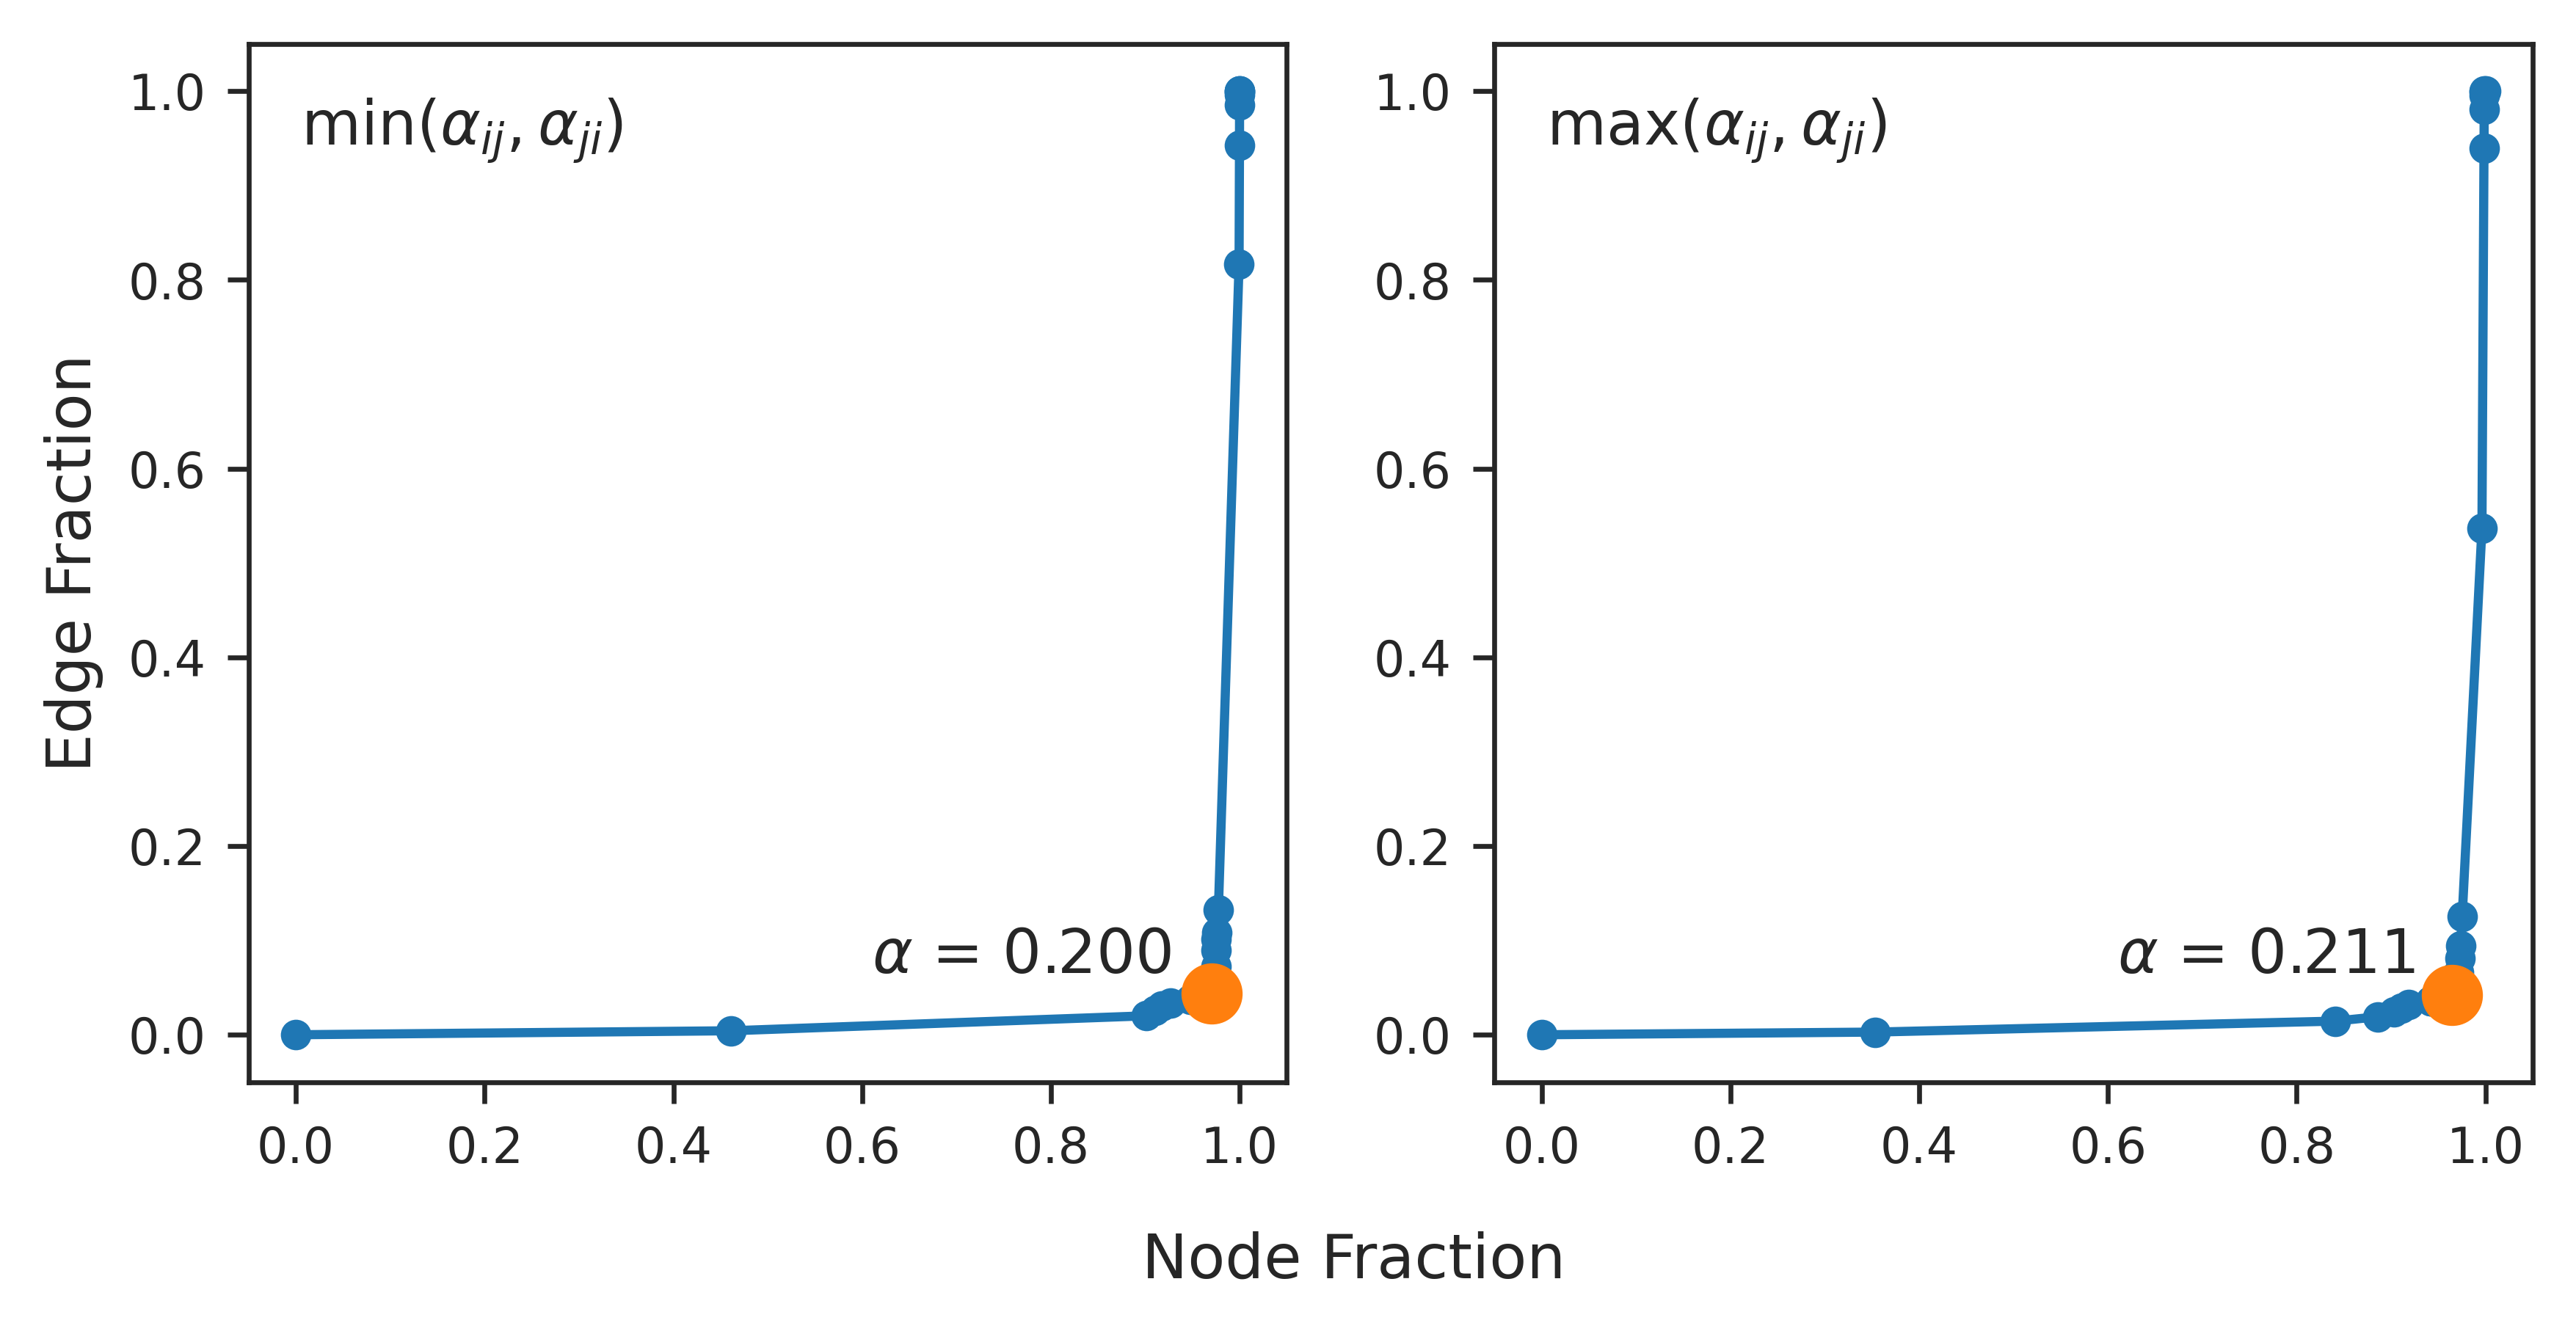
\includegraphics[width=1\textwidth]{alpha_tables.png}
  \caption{\textbf{Optimal alpha selection process}. To define the optimal alpha value to sparsify the chromosome-level network, local search is performed. In the panels, sets of points tested to find the optimal alpha value for chromosome 1 of IMR90 cells at 10 kb resolution, processed using 200 Mb as distance threshold, 0 as quantile threshold. On the left, local search for the optimal value using maximal alphas. On the right, local search for the optimal value using minimal alphas.}
  \label{fig:alphas}
\end{figure}

\subsection{Pixel sparsification}

After computing the sparsification scores for the filtered pixels and the appropriate alpha thresholds, the actual sparsification step can be conducted. In figure \ref{fig:sparsification}, some statistics regarding pixel number and genomic distance for files which were sparsified using the optimal alpha values are reported. The only combinations of parameters which are shown are those which were considered appropriate in the filtering step; as was previously noted, those combinations yielded very similar filtering results, therefore it is not surprising that the same holds true for the sparsification step.

In the top panel, it can be seen that sparsification leads to a drastic reduction in the number of pixels retained; on average, only 5\% of the pixels are kept. This holds true for both the minimal alpha and the maximal alpha case, which is partially to be expected considering how similar the thresholds tend to be. In the central panel, the mean genomic distance fold change is shown; a very strong decrease can be observed, which corresponds to the average genomic distance being reduced by 95\%, which is constant for both alpha modalities as well as all parameter combinations. Finally, in the bottom panel, the median genomic distance is shown; once again, there is a strong reduction, though less severe, averaging at 80\% of the filtered measure, regardless of alpha modality and parameter combination.

It is worth noting that, even though in terms of fold change there is a drastic reduction in the distance statistics, in terms of absolute values, those statistics are still quite high; the median value for the mean genomic distance after sparsification is 590 kb, while for the median it is 400 kb. Moreover, the distances obtained after sparsification, even for the worst file (95 kb), are compatible with the range in which most enhancer-promoter interactions are expected to be found, which are, for most applications, the interactions of interest.

% Plot number of pixels as function of parameters
% Plot distance of pixels as function of parameters
\begin{figure}[ht]
  \centering
  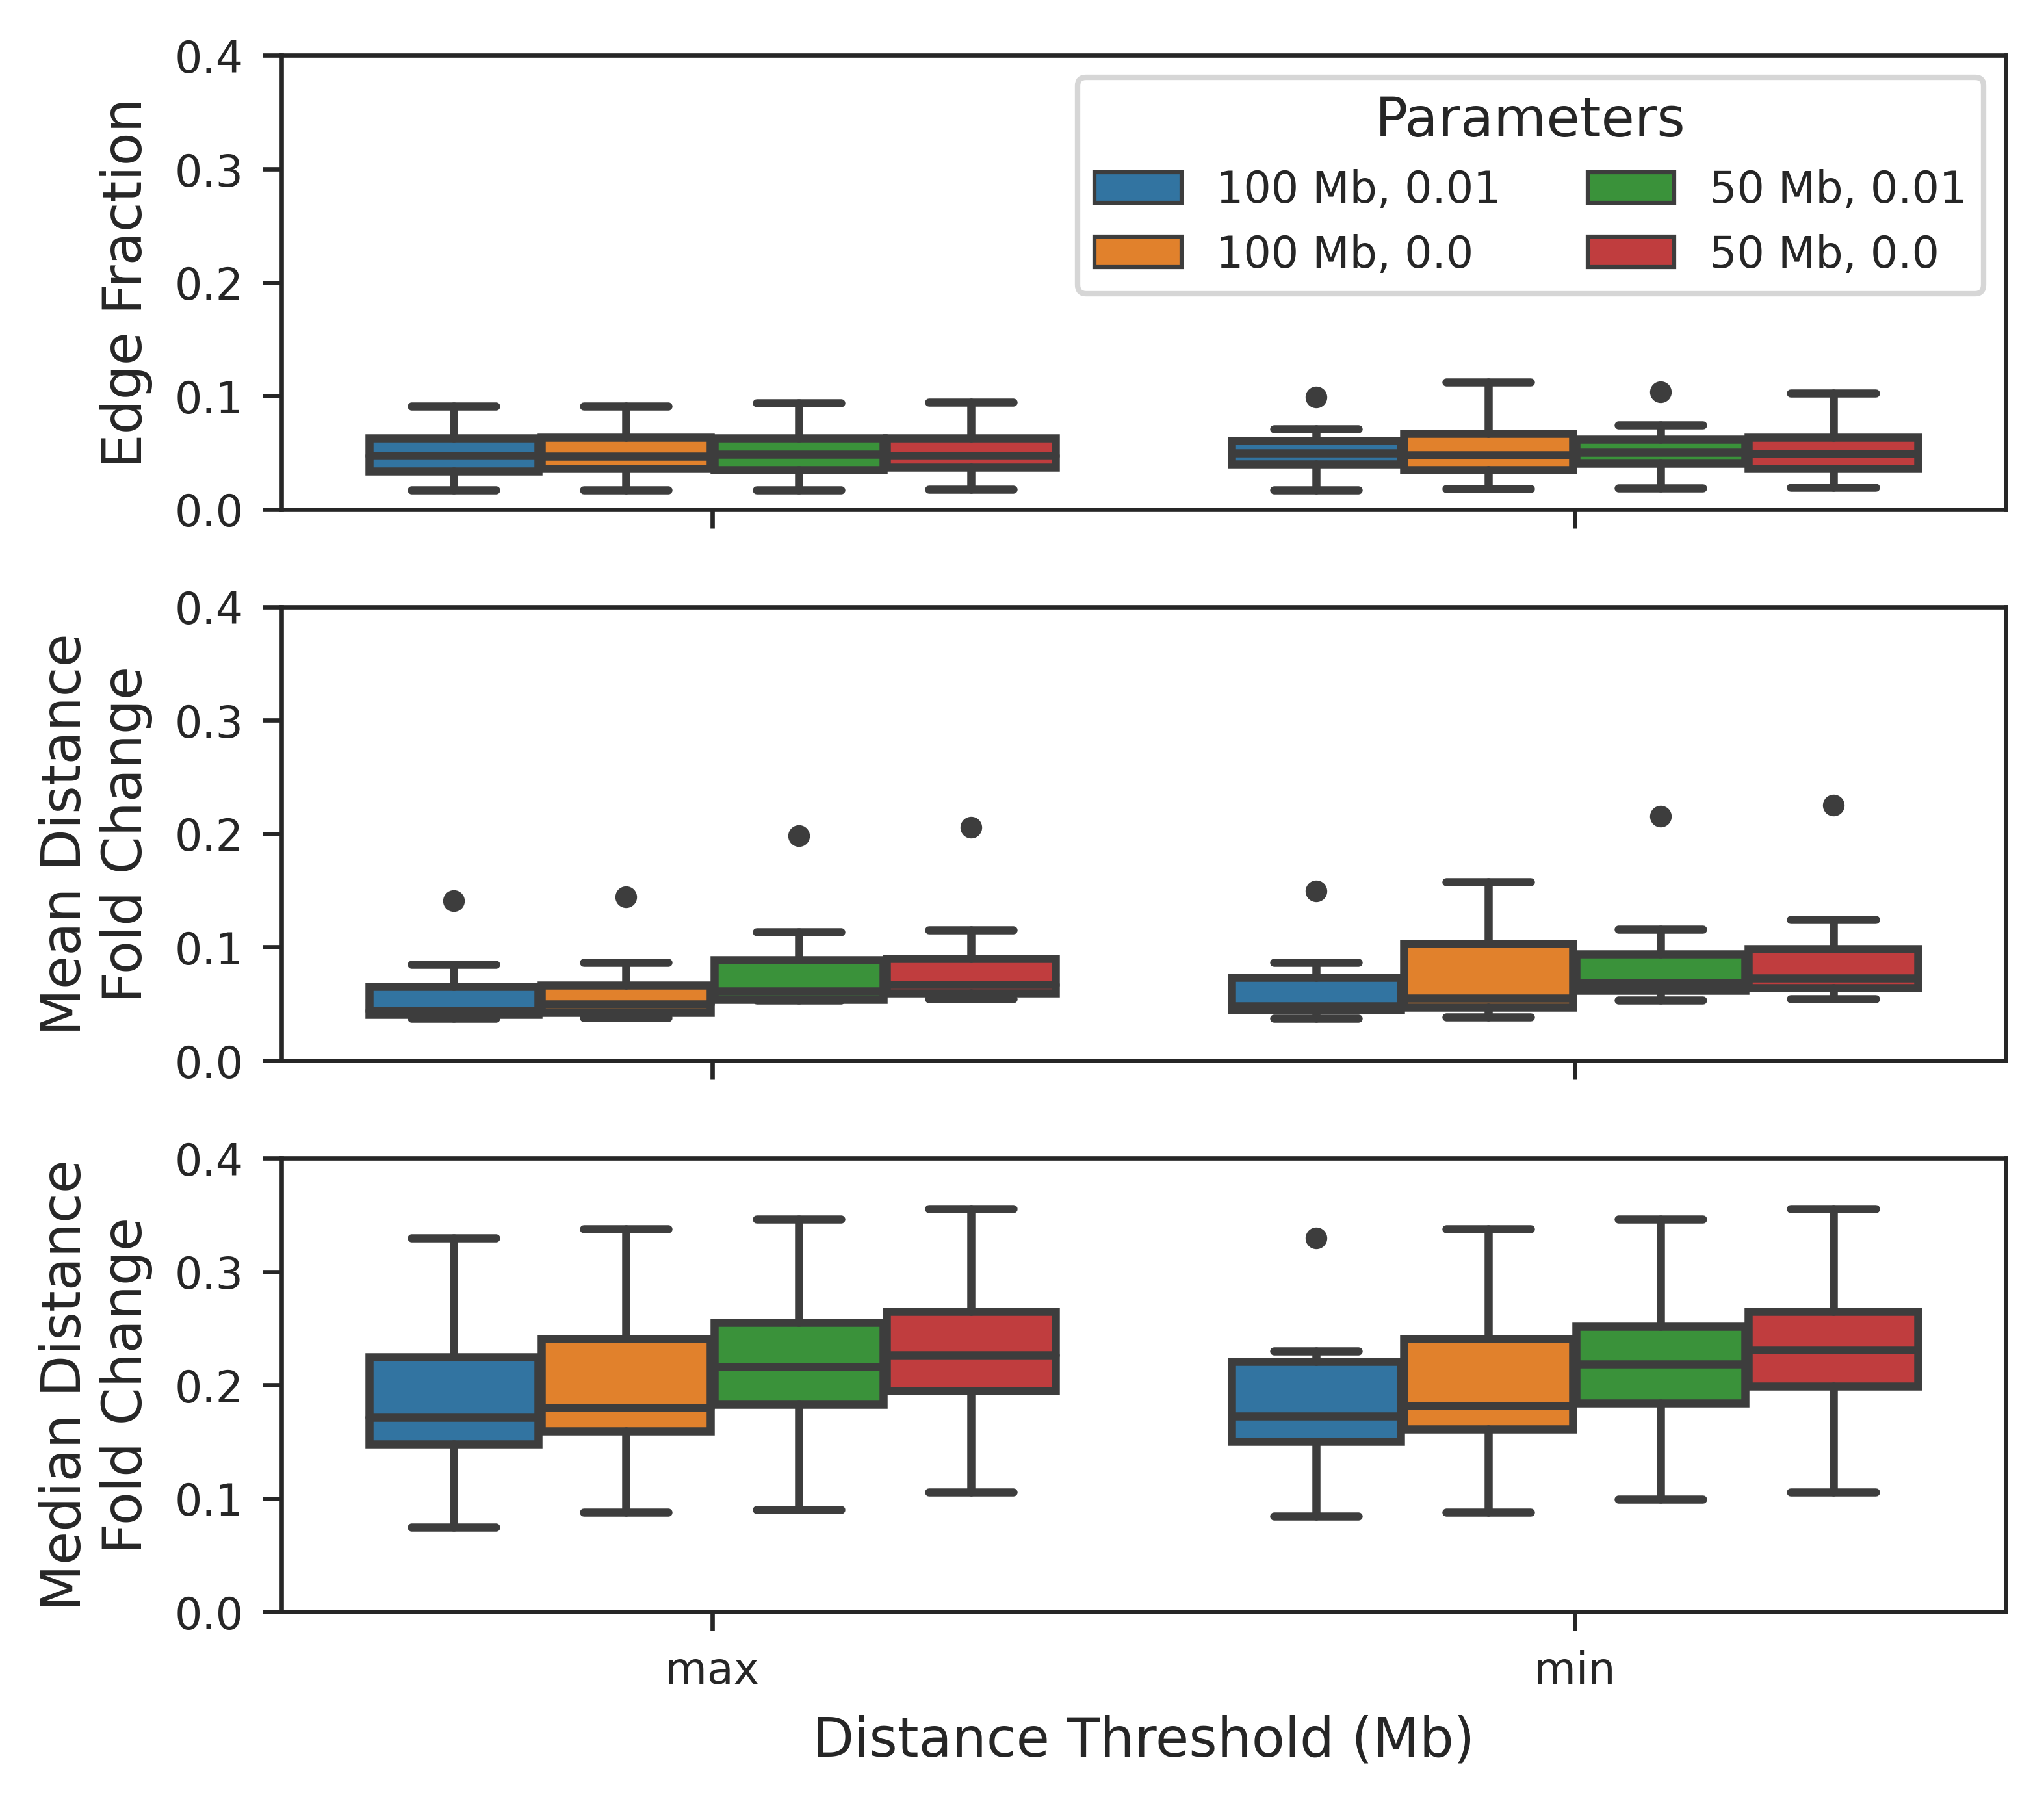
\includegraphics[width=0.8\textwidth]{sparsification_stats.png}
  \caption{\textbf{Changes in pixel number and distance statistics after sparsification.} Comparison of the changes in edge number and distance statistics after sparsification using optimal alpha value threshold on all files at 5 kb resolution. In each panel, the boxplots are divided into two groups, respectively using minimal and maximal alphas. Each group is composed of the boxplots corresponding to the combinations of parameters which were previously deemed appropriate in the filtering subsection. At the top, fraction of chromosomal pixels remaining after sparsification. In the middle, fold change between sparsified pixels mean genomic distance and filtered pixels mean genomic distance. At the bottom, fold change between sparsified pixels median genomic distance and filtered pixels median genomic distance.}
  \label{fig:sparsification}
\end{figure}

% Plot variation coefficient with other tools too
% Plot expected interaction distance with respect to other tools


\section{Pixel preprocessing performance}
Most of the operations performed by the package could probably be applied on an entire chromosome at once, given that enough Random Access Memory (RAM) is available to store it and the results in memory; though this might be true, it is a rather brute force method which relies on having access to a fairly high-end machine or a cluster. Given that the package aims to make network analysis of Hi-C data accessible, this is definitely not an option. In order to make the processing manageable even on lower-end laptops, the entirety of it, from filtering to sparsification, is conducted in chunks. By chunking the process, the RAM footprint decreases, allowing it to adapt it to system specifics. While chunking itself does not speed up the computation, it must be noted that a chunked procedure is more amenable to parallelization, therefore it could result in significantly faster runtimes with respect to a non-chunked procedure. 
In the next subsections, benchmarking on both computational runtime as well as RAM usage are required.

\subsection{Time benchmark}

% Plot number of filtered pixels vs time (linear)
\begin{figure}[ht]
  \centering
  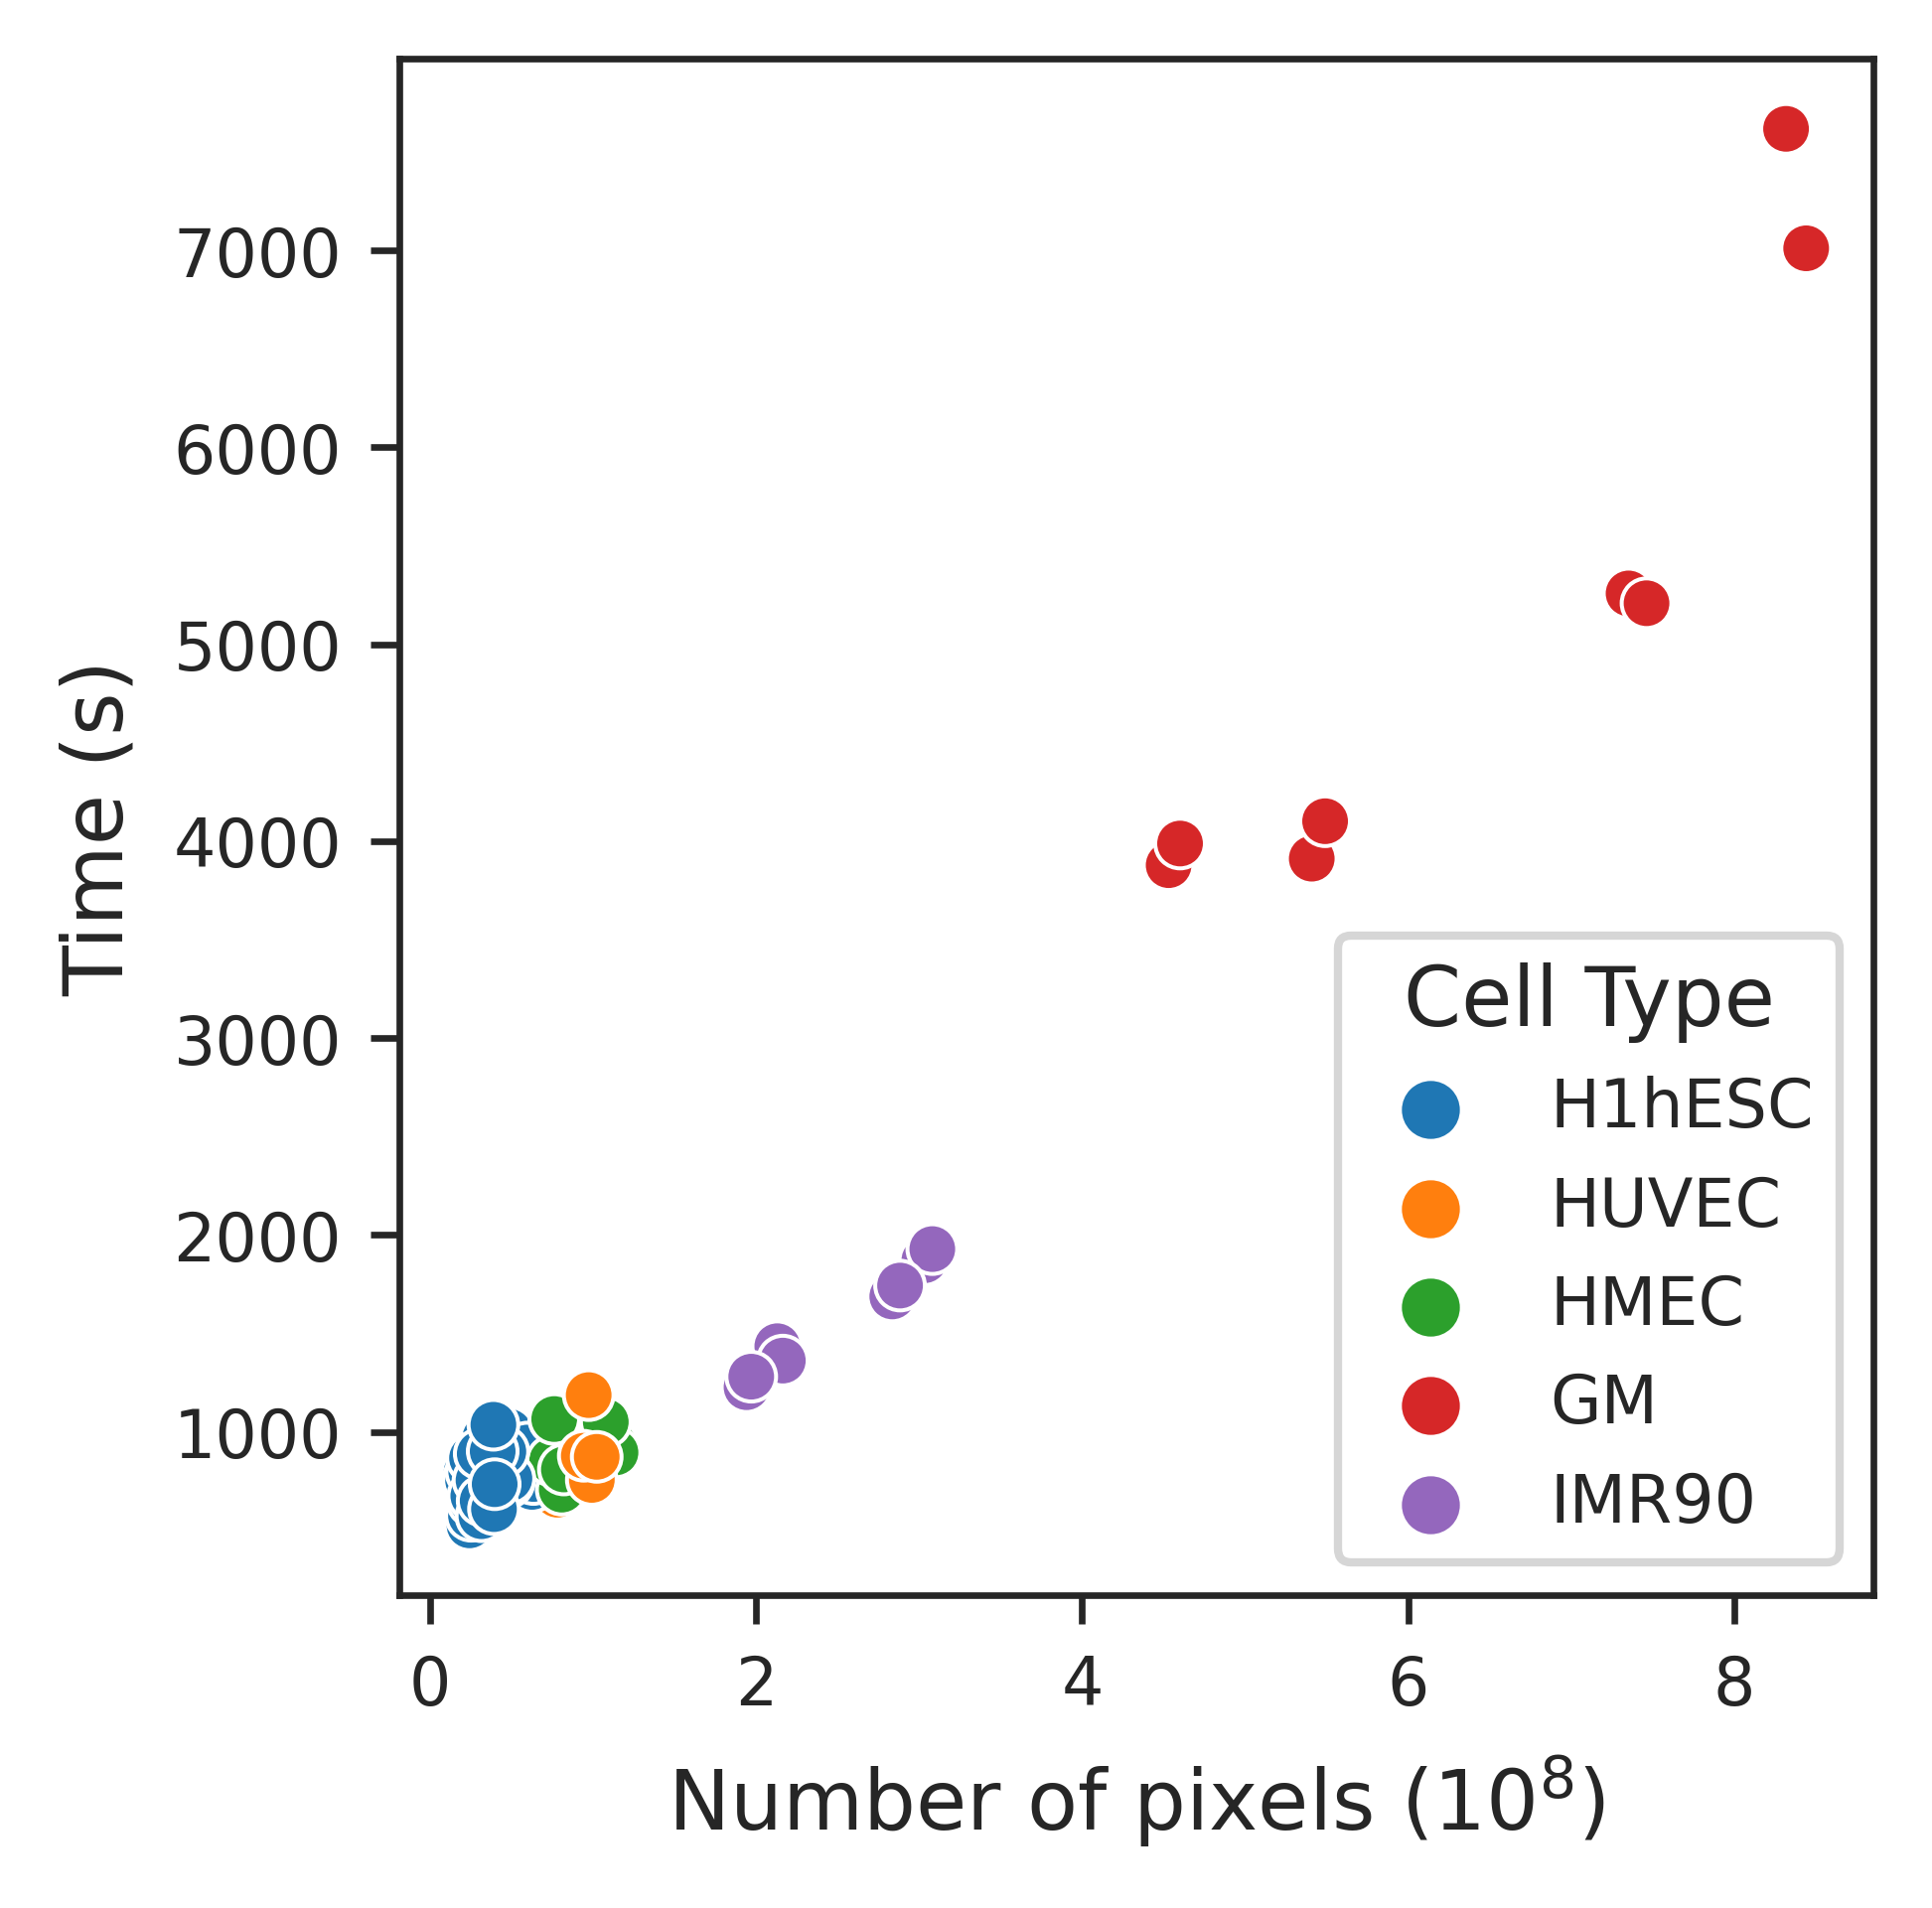
\includegraphics[width=1\textwidth]{time_benchmark.png}
  \caption{\textbf{Pixel preprocessing time benchmark}. A) Time required to compute the sparsification scores for each file, with different parameter combinations, as a function of the number of pixels remaining after filtering. As one might expect, there appears to be a linear correlation between number of pixels to process and time required. B) Comparison of the time required by HiCONA and common loop-callers to process an IGM90 cells replicate file (4DN data portal id: 4DNFIAAUZ7EP). Runtimes for the loop-callers were obtained from Forcato et al., 2017. The file was processed by HiCONA using a distance threshold of 100 Mb and a quantile threshold equal to 0.01. HiCONA is much faster than all the loop-callers.}
  \label{fig:timebenchmark}
\end{figure}

Time benchmarking was performed by analyzing the wall-time required to process each file using a certain set of parameters. The sparsification scores computation step is by far the most computationally intensive step, to the point where the time required by the other operations is basically negligible; in fact, as shown in figure \ref{fig:timebenchmark}A, the time required for the file to be processed correlates with the number of pixels remaining after the filtering step. From the sparsification algorithm we expect the relation to be linear (which is indeed the case), since the number of integrals to be computed is twice the number of pixels remaining after filtering. Still, it must be considered that, although the normalized counts are floating point numbers, they are obtained by taking the log2 of a fraction whose terms are integers; not only that, the values which the denominator can take are rather limited, very rarely exceeding 100. For this reason, in actuality, the pool of normalized values is smaller than it might seem which, combined with the fact that most integrals are repeated, makes it possible to drastically reduce the number of integrals computed. Since each integral only depends on the number of neighbors and the normalized edge weight (see \ref{par:sparscore}), a \texttt{pandas.DataFrame.groupby()} on those two columns was performed in order to obtain the set of unique combinations; then, after computing the integral for each combination, the values are associated back to the pixels by using a \textit{left-outer-join} merge. Though the same integral is computed multiple times if it appears in multiple chunks of the table being processed, this way it is possible to compute, on average, only 65,000 integrals per million of filtered pixels, maintaining linearity while reducing the slope.

From figure \ref{fig:timebenchmark}A, it is also possible to see the time it took for the each file to be processed (using the 4 combinations of parameters which were considered viable); standard-sized files, such as H1hESC, HUVEC and HMEC, are processed in roughly 30 minutes, while GM and IMR90, which are usually used as examples of very big files for Hi-C benchmarking, are still processed in little over two hours at most. 

In figure 4.6B, the speed of HiCONA was compared to the most common loop-callers. One of the replicates of IMR90 cells (4DN data portal id: 4DNFIAAUZ7EP), was processed with the standard pipeline for each tool. For the loop-callers, the time to perform normalization and analysis was obtained from Forcato et al., 2017 [https://pubmed.ncbi.nlm.nih.gov/28604721/]. The file was processed by HiCONA using a distance threshold of 100 Mb and a quantile threshold equal to 0.01. For HiCONA, the initialization and filtering steps are included too since they have negligible runtime with respect to sparsification. It can be seen that HiCONA is much faster than all loop-callers, with diffHic being the only one with a comparable runtime.

% From the right panel of figure \ref{fig:timebenchmark}, it is visible that, for each genomic distance threshold applied, there is a linear dependency between number of filtered pixels and required time, though these dependencies can have quite different slopes. In general, it seems that, the lower the genomic threshold, the steeper the slope; though not fully understood, it seems that lower genomic threshold lead to the presence of more unique integrals, therefore causing the runtime to be slower.

\subsection{Memory benchmark}

RAM usage was tested only on a subset of the files since \texttt{memory\_profiler}, the package which was used, computes memory usage by pausing script execution every 0.1 seconds. In figure \ref{fig:memorybenchmark}, RAM usage overtime for the preprocessing of all chromosomes of a single file, using one set of parameters, is shown. In the figure, every pair of dashed red lines corresponds to the interval in which the sparsification scores for a chromosome are computed. It is thus worth noting that the time spent for operations other than sparsification scores computation corresponds exclusively to the interval before the first red line and the interval after the last one; as mentioned in the previous subsection, this amount of time is basically negligible compared to the one used for sparsification.

% Plot of the run of a single file using memprof
\begin{figure}[h]
  \centering 
  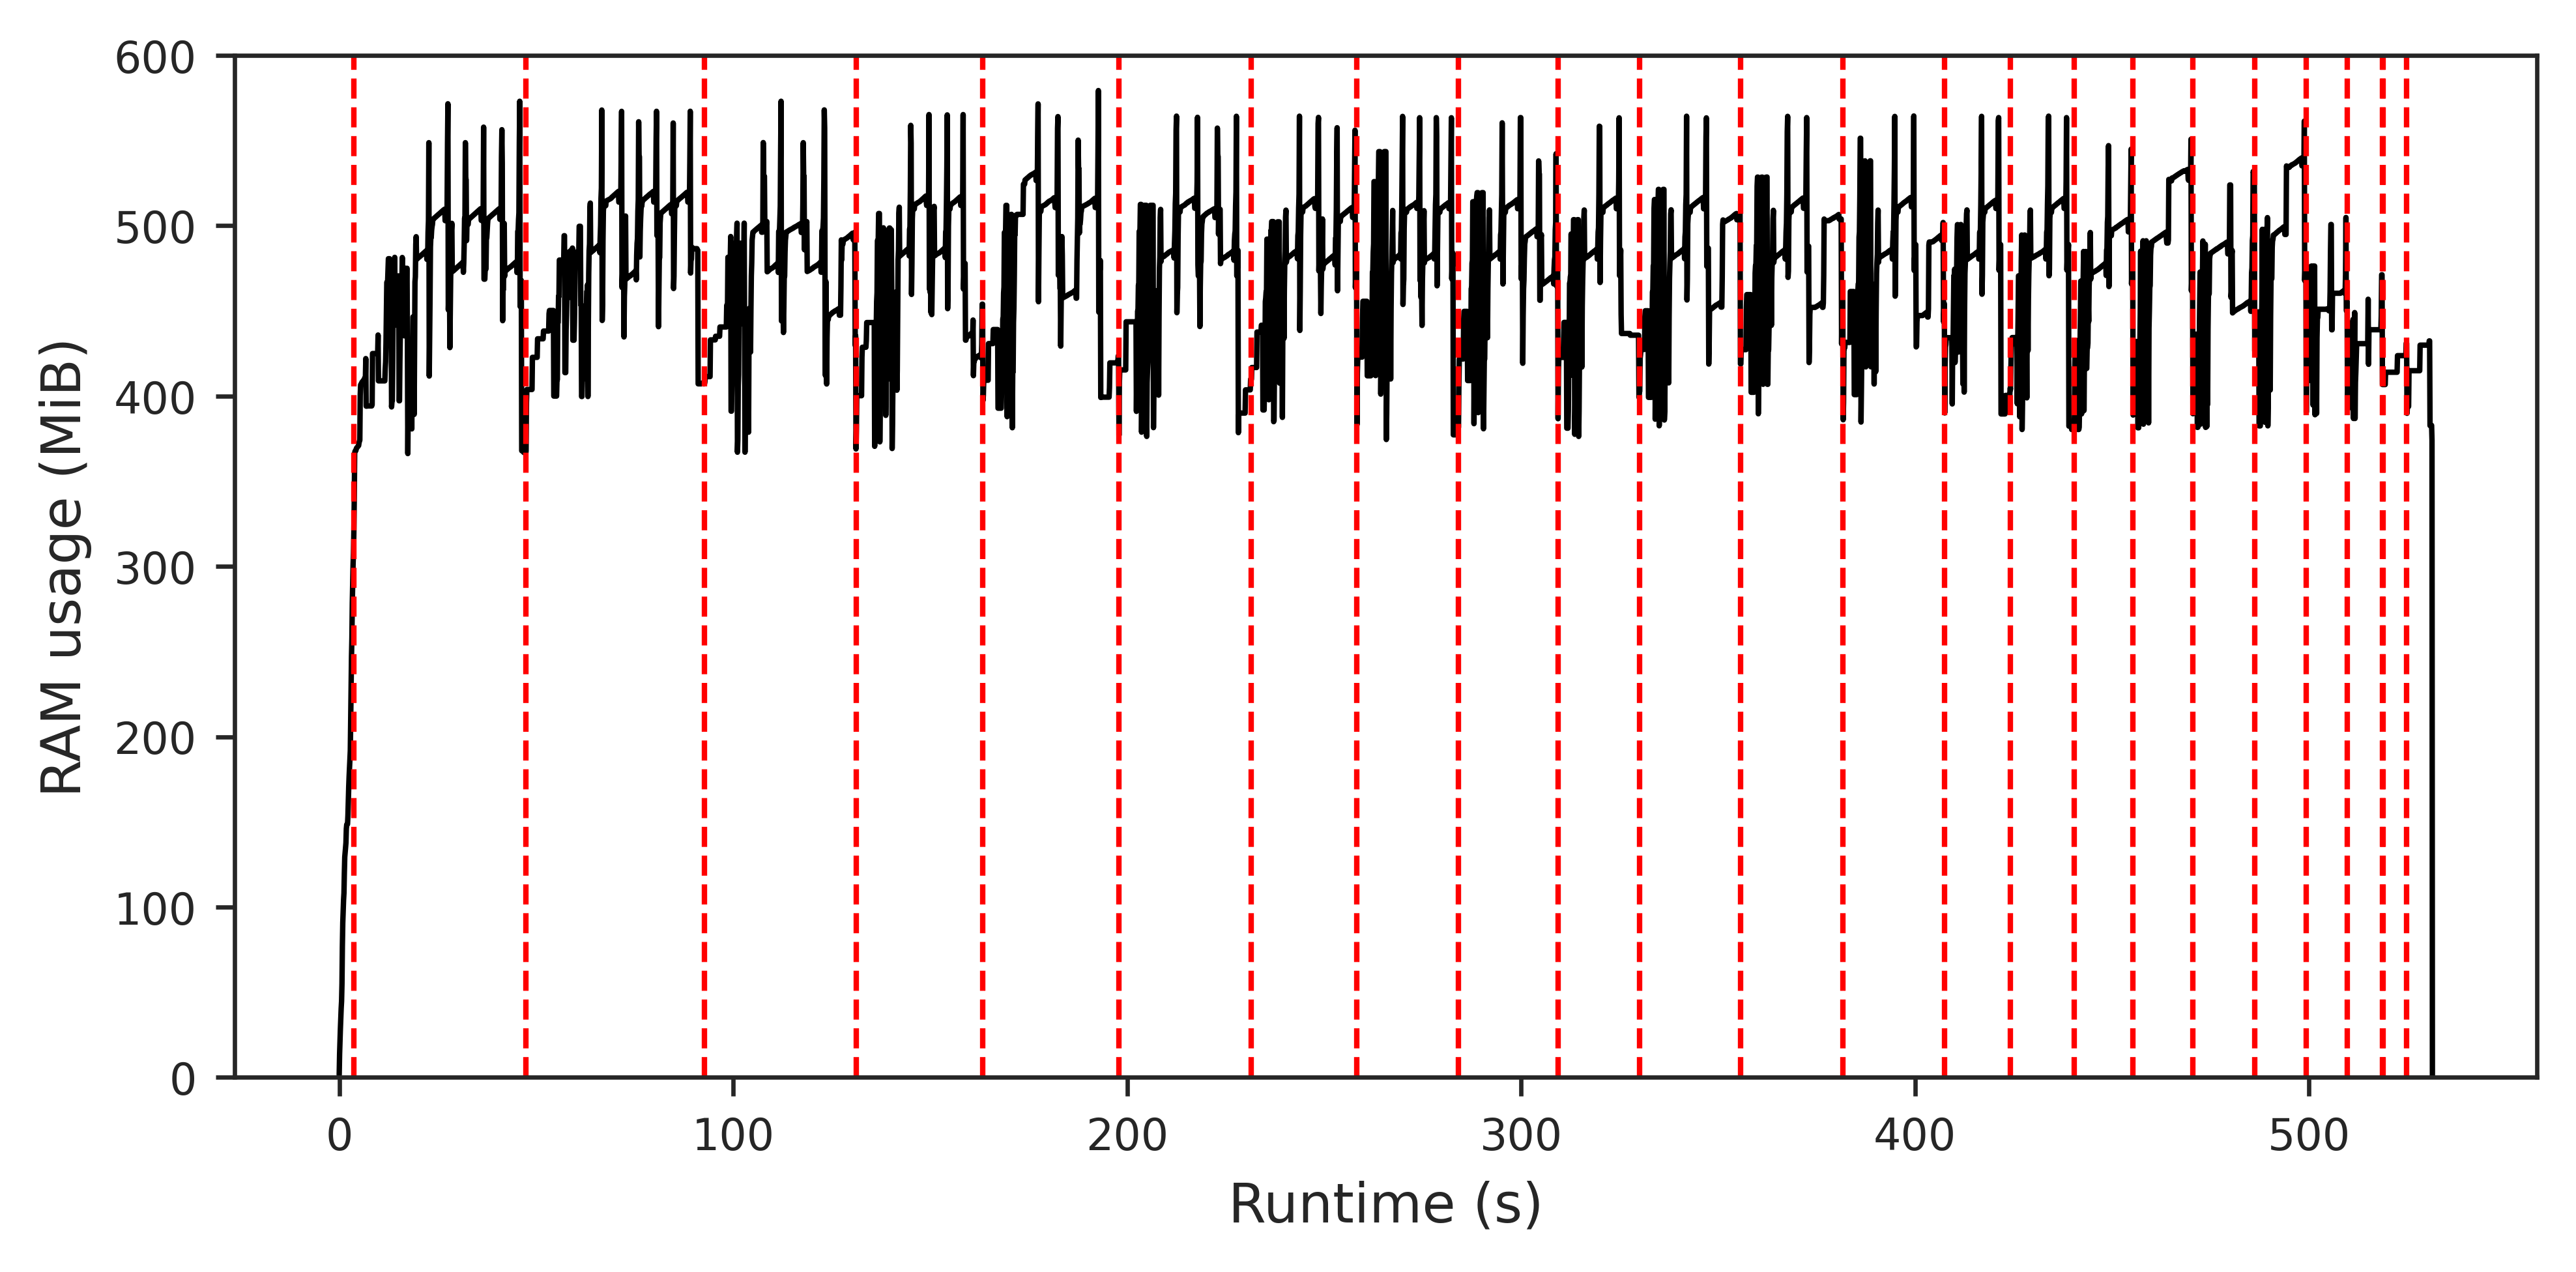
\includegraphics[width=1\textwidth]{memory_benchmark.png}
  \caption{\textbf{Preprocessing RAM usage overtime}. Plot of Random Access Memory usage during the preprocessing procedure. Runtime is expressed in seconds, while memory usage is expressed in MebiBytes (1 MiB = $2^{20}$ bytes). The area included between two red dashed lines corresponds to the sparsification scores computation for a chromosome. In the figure, the RAM usage overtime for IMR90 cells at 10 kb resolution, processed using 200 Mb as distance threshold, 0 as quantile threshold, is shown.}
  \label{fig:memorybenchmark}
\end{figure}

It can be seen that the program initially loads some objects into memory, reaching around 400 MiB of RAM, then sparsification causes fluctuations of around 200 MiB, for a maximum RAM usage of less than 600 MiB. The memory load prior to sparsification can vary slightly depending on file properties, while the amplitude of the fluctuations during sparsification is constant, since it uniquely depends on the chunk size used during processing (by default, 1 million pixels per chunk). In fact, each peak corresponds to a chunk being loaded into memory. Therefore, HiCONA does indeed allow to process any file using a very low, fixed, amount of RAM.

\section{Pixel preprocessing biological validation}

Even though the procedure might work for network analysis purposes, that does not mean that the procedure is able to yield significant biological results. Some form of validation is needed, to show that the networks have features which are amenable to perform biologically meaningful analyses. One feature was already discussed, that being the average pixel genomic distance, which was shown to be compatible with the analysis of promoter-enhancer interactions. In the following subsections another form of validation will be discussed, which is the consistency of the procedure on biological and technical replicates.

\subsection{Consistency on replicates}
% Plot Jaccard index on replicates 
% Plot Jaccard index vs file size pre and after processing
% Plot Jaccard index with respect to other tools

Ideally, data generated from replicates should have a high degree of concordance if the biological procedure is consistent and stable enough; this concordance should be maintained, if not increased, by the following processing steps in order to obtain robust and generalizable results. To analyze this concordance, a measure of similarity must be introduced; considering the different sizes of the networks, a good choice is the Jaccard index, which is defined as the cardinality of the intersection of the two networks over the cardinality of their union (i.e. the number of shared edges over the number of all edges, regardless of their weights). All technical and biological replicates from both IMR90 and GM cells at 5 kb resolution were processed using different combinations of parameters; the Jaccard indexes were computed just after the filtering step and after the sparsification procedure.

\begin{figure}[h]
  \centering 
  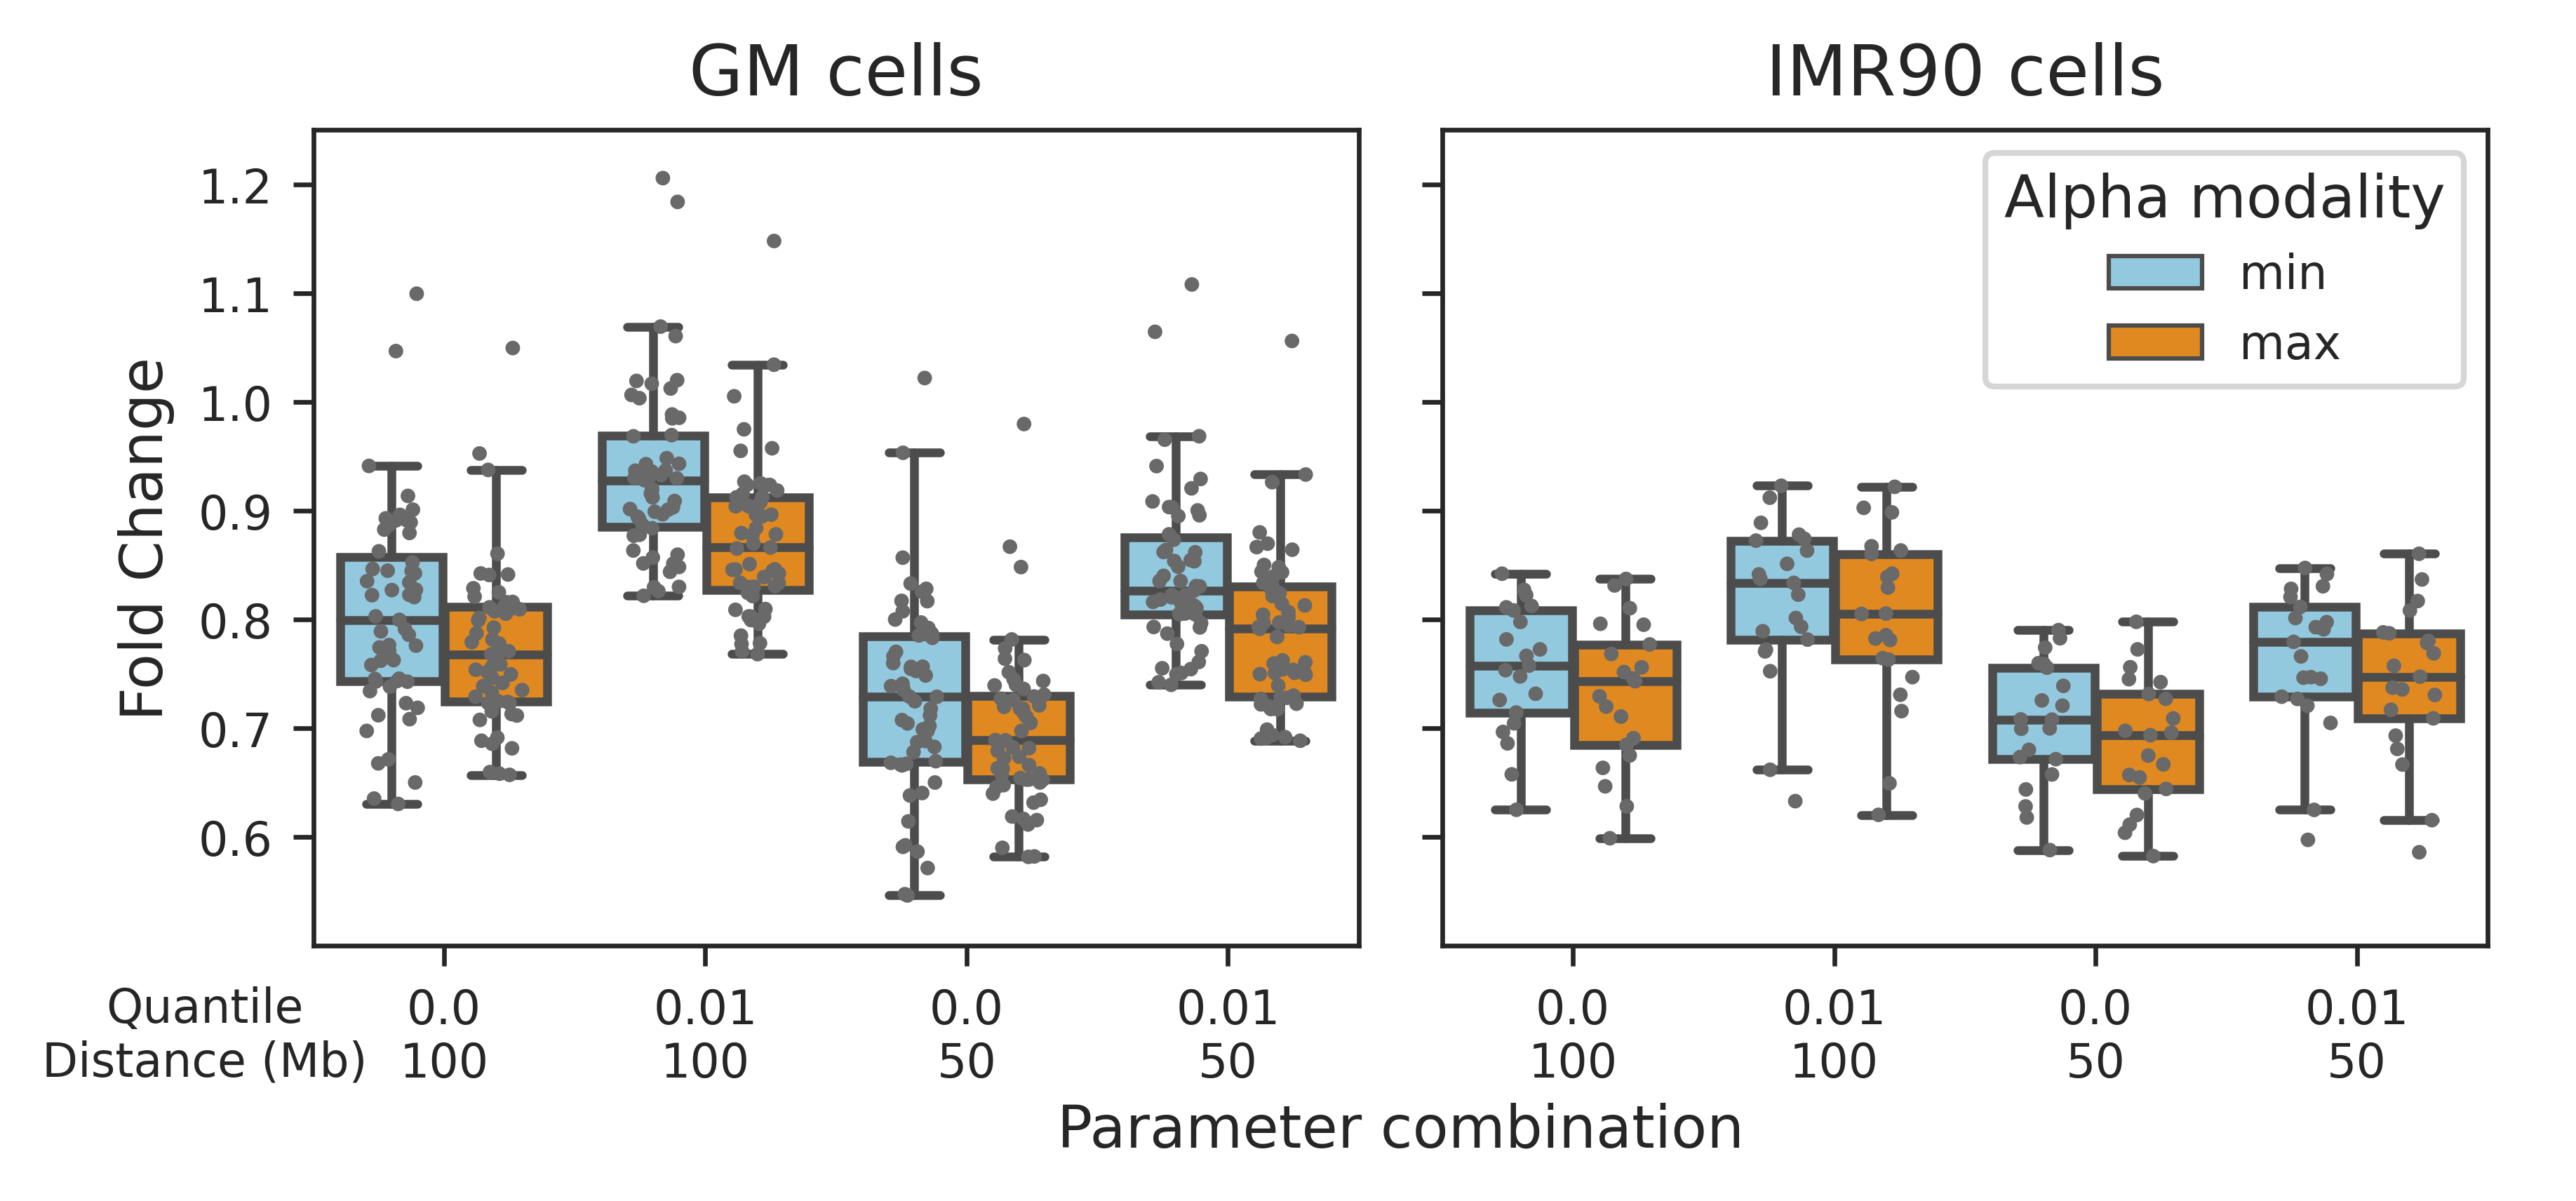
\includegraphics[width=1\textwidth]{fold_changes.png}
  \caption{\textbf{Jaccard index fold change}. Fold changes between Jaccard index after sparsification and Jaccard index after normalization. The distribution of the fold changes is shown for each combination of parameters used during processing, and for both alpha modalities. In the left panel the fold changes for GM cells, in the right panel those for IMR90 cells. The combination of parameters with distance threshold equal to 100 Mb and percentile threshold equal to 0.01 is the one consistently yielding higher fold changes (and thus higher similarity).}
  \label{fig:foldchanges}
\end{figure}

For GM cells, the Jaccard indexes among filtered replicates spanned the range 0.07-0.17, while those for the sparsified replicates (regardless of minimal or maximal optimal alpha), spanned the range 0.055-0.15. No pattern was found in the distribution of the Jaccard indexes, even considering different filtering parameters. For IMR90 cells, the Jaccard indexes among filtered replicates spanned the range 0.055-0.17, while for the sparsified replicates (again, regardless of alpha) the range was 0.035-0.13. In this case a loose bimodal distribution was visible, with Jaccard indexes being close to either of the range limits. Though there is no real metric to define what a good Jaccard index among replicates should be in this situation, the values seem fairly low. As previously described though, the used thresholds are very loose, to the point were the datasets are very similar to the raw contact matrices without self-looping pixels and inter-chromosomal pixels; this means that, for what concerns intra-chromosomal pixels, the Jaccard indexes of the raw file themselves are likely low, suggesting that the consistency is low due to either the biological procedure or the steps to create the contact matrix.

Having asserted that the starting Jaccard indexes are fairly low, the pressing point for the sparsification procedure becomes to try and preserve, or ideally increase, these Jaccard values. To analyze this aspect, the fold changes between Jaccard indexes computed on the sparsified files and those computed on the filtered files are shown in figure \ref{fig:foldchanges}. To test whether any of the combinations of parameters yields, on average, a different fold change with respect to the others, Friedman test was performed. Friedman test is a non-parametric test for the comparison of multiple groups of paired data. For IMR90 cells, the p-value of the test is in the order of $10^{-12}$ for both minimal and maximal alphas; for GM cells, the p-values for minimal and maximal alphas were in the order of $10^{-33}$ and $10^{-32}$, respectively. Considering that all p-values were significant by a long margin, post-hoc analysis was performed to define which sets of parameters actually have different means. To do so, Wilcoxon Signed-Rank test, a non-parametric test to compare two groups of paired data, was used; the p-values were then corrected using Bonferroni correction (which in this case meant multiplying by 24, since 6 pairs of groups are tested for each of the 4 conditions). For all conditions, all pairs of combinations of parameters resulted significantly different, aside from the pair composed of the combinations "distance threshold equal to 100 Mb, quantile threshold equal to 0" and "distance threshold 50 Mb, quantile threshold equal to 0.01", which were not significant for IMR90 cells. 

% 1.2732112864879016e-12 IMR90 max
% 1.686243757817196e-12 IMR90 min
% 1.3594150523742334e-33 GM min
% 1.324003892549082e-32 GM max

% GM max
% 2.6582763710725764e-09, 
% 2.6582763710725764e-09, 
% 0.012164962590814125, 
% 2.6582763710725764e-09, 
% 2.6582763710725764e-09, 
% 2.6582763710725764e-09

% GM min 
% 2.6582763710725764e-09, 
% 2.6582763710725764e-09, 
% 6.158779753916076e-06, 
% 2.6582763710725764e-09, 
% 2.6582763710725764e-09, 
% 2.6582763710725764e-09

% IMR90 min 
% 2.288818359375e-05,
% 2.288818359375e-05, 
% 2.13116455078125, 
% 2.288818359375e-05, 
% 2.288818359375e-05, 
% 2.288818359375e-05

% IMR90 max
% 2.288818359375e-05, 
% 2.288818359375e-05, 
% 0.24300384521484375, 
% 2.288818359375e-05, 
% 2.288818359375e-05, 
% 2.288818359375e-05

From these results we derive that the combination of distance threshold equal to 100 Mb and quantile threshold equal to 0.1 is the one leading to the smallest reductions in Jaccard index during the sparsification procedure. In fact, in IMR90 cells, this threshold yielded an average fold change of 0.805 using maximal alphas, 0.834 using minimal alphas; for GM cells the thresholds for maximal and minimal alphas were 0.866 and 0.928, respectively. While there is still a fairly wide spread of points even for the best combination of parameters, it is worth noting that some replicates can have up to two orders of magnitude of pixels less than others, in which case, it seems hard for any set of parameters to close the gap. Overall, it seems that the sparsification procedure, given the right parameters, is able to process replicates with a high degree of similarity.

In figure \ref{fig:jaccardtools}, the consistency of HiCONA was compared to the consistency of some common loop-callers. This was done by comparing their Jaccard indexes on replicates of IMR90 cells and GM12878 cells. All replicates were processed using the suggested procedure for each loop-caller; the data was obtained from Forcato et al., 2017. The files were processed by HiCONA using a distance threshold of 100 Mb and a quantile threshold equal to 0.01, since it is the combination of parameters which seems to perform the best in terms of Jaccard fold change. It can be seen that the various loop-callers have quite different Jaccard indexes, though all of them are quite low. Although HiCONA did not produce the highest values, it is the tool which is consistently higher than all others, regardless of whether minimal or maximal alpha was used.

\begin{figure}[h]
  \centering 
  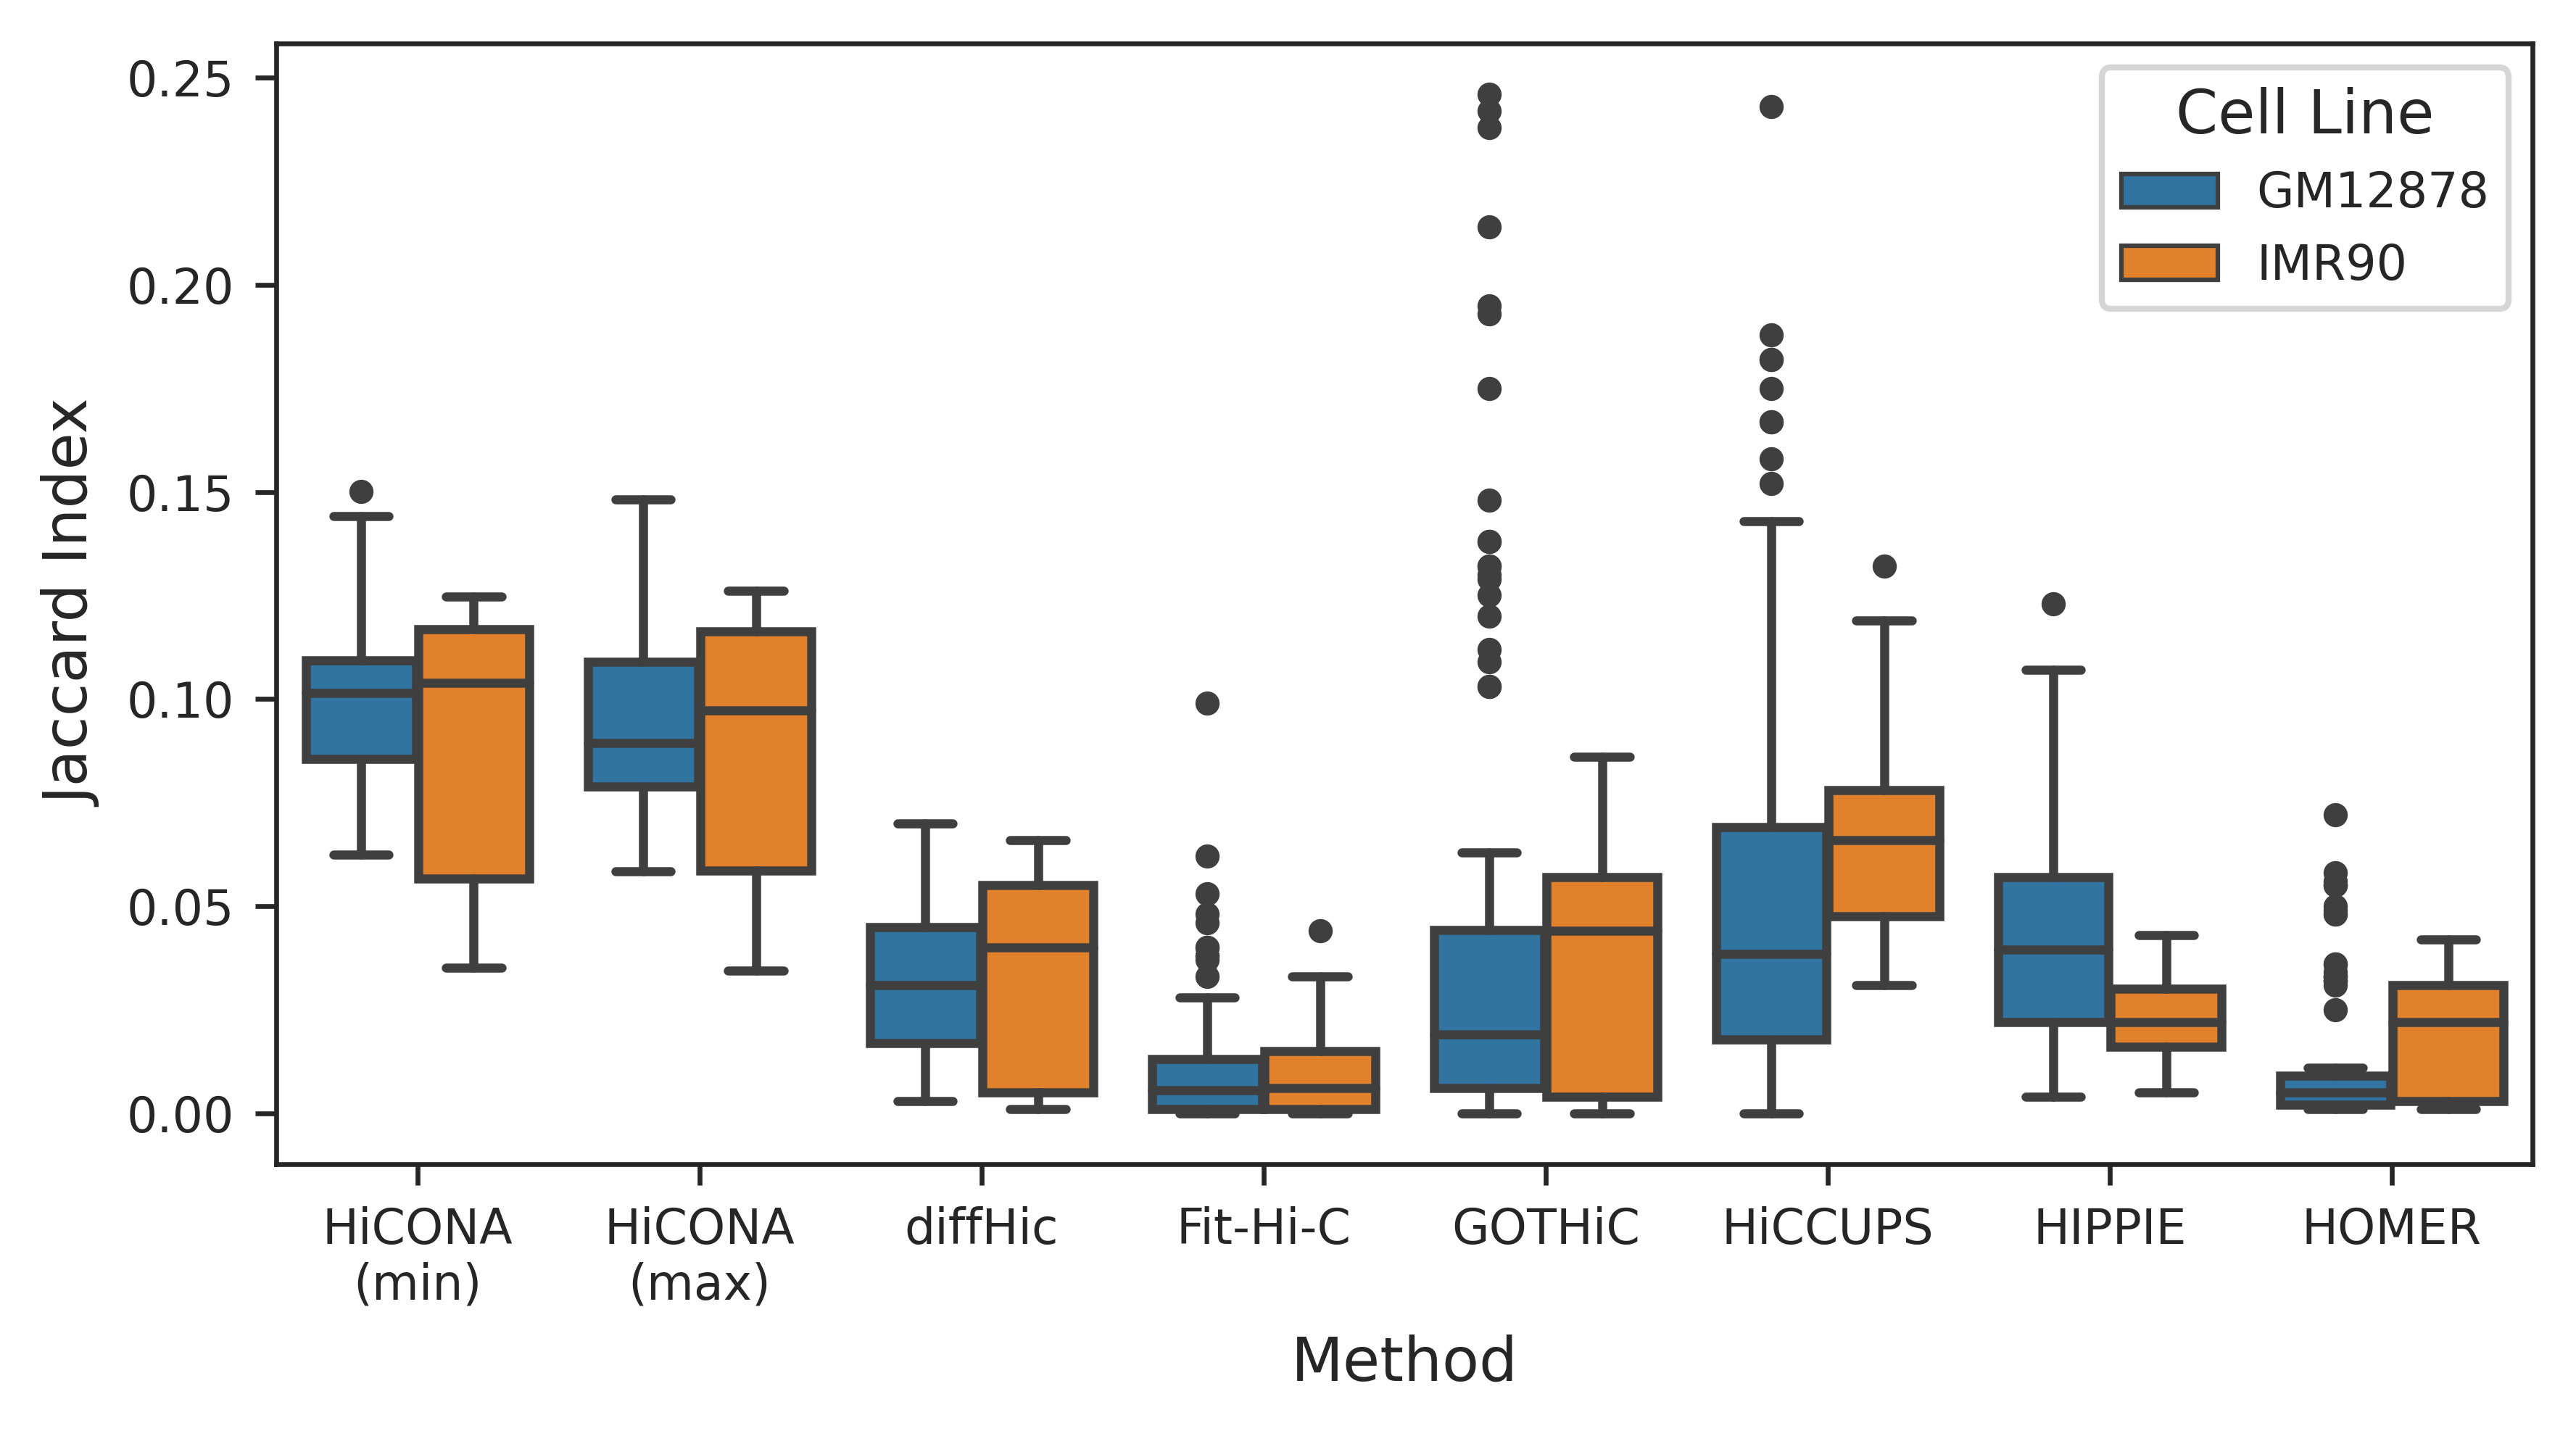
\includegraphics[width=1\textwidth]{jaccard_tools.png}
  \caption{\textbf{Comparison of Jaccard indexes from HiCONA and loop-callers.} Jaccard indexes on replicates of IMR90 cells and GM12878 cells were computed for both HiCONA and common loop-callers. All files were processed using the suggested procedure for each loop-caller. For HiCONA, distance threshold of 100 Mb and quantile threshold equal to 0.01 were used. HiCONA seems to be consistently higher than all other tools. Data for the loop-callers from Forcato et al., 2017.}
  \label{fig:jaccardtools}
\end{figure}

% \subsection{Functional annotations enrichment}
% Plot edge annotation fraction
% Plot edge annotation enrichment



% \section{Network analysis}
% \subsection{Node-label permutations}
% Plot node-label permutation for 1 file, chromosome-wise (maybe new ann)

% ? Plot Hi-C maps at different steps
